\documentclass[pdf,aspectratio=169]{beamer}
\usetheme{Copenhagen}
\usepackage{multicol, latexsym, amsmath, amssymb}
\usepackage{smartdiagram}
\usepackage{subcaption}
\usepackage{colortbl}
\usepackage{svg}
\setbeamertemplate{navigation symbols}{}
\newcommand{\z}{\mathbf{z}}
\newcommand{\uout}{u_{out}}
\newcommand{\vout}{v_{out}}
\newcommand{\uoutdum}{u_{out}^{dum}}
\newcommand{\uinplus}{u_{in}^{+}}
\newcommand{\uinminus}{u_{in}^{-}}
\newcommand{\winl}{w_{in}^{l}}
\newcommand{\win}{w_{in}}
\newcommand{\uin}{w_{in}}
\newcommand{\vin}{v_{in}}

\DeclareMathOperator*{\plusrightarrow}{\ensuremath{\xrightarrow{+}}}
\DeclareMathOperator*{\minusrightarrow}{\ensuremath{\xrightarrow{-}}}
\DeclareMathOperator*{\plusleftarrow}{\ensuremath{\xleftarrow{+}}}
\DeclareMathOperator*{\minusleftarrow}{\ensuremath{\xleftarrow{-}}}
\renewcommand<>\rowcolor[1]{\only#2{\\[-\normalbaselineskip]\beameroriginal\rowcolor{#1}}}
\title{Scalable Pipelines for Lexical \& Semantic Text Reuses}
\subtitle[]{Workshop on Text Reuse in the Eighteenth Century}
\setbeamertemplate{footline}[text line]{%
    \parbox{\linewidth}{\vspace*{-8pt}\hfill\hfill\insertframenumber\,/\,\inserttotalframenumber}}
\author{Ananth Mahadevan}
\institute{Computer Science Department\\University of Helsinki}

\date{2nd May 2024}

\AtBeginSection[]{
  \begin{frame}
  \vfill
  \centering
  \begin{beamercolorbox}[sep=8pt,center,shadow=true,rounded=true]{title}
    \usebeamerfont{title}\insertsectionhead\par%
  \end{beamercolorbox}
  \vfill
  \end{frame}
}

\begin{document}
\begin{frame}
    \titlepage
\end{frame}

\begin{frame}
    \frametitle{Contents}
    \
    \tableofcontents
\end{frame}


\section{Lexical Text Reuses}

\begin{frame}
  \frametitle{Lexical Pipeline}
  \begin{enumerate}
    \item Identify lexical text reuses
    \begin{itemize}
      \item BLAST
    \end{itemize}
    \item Extract-Transform-Load (ETL)
    \begin{itemize}
      \item De-fragment
      \item Cluster
      \item Identify
    \end{itemize}
    \item Locke Quotes Task
    \begin{itemize}
      \item Task-specifc data
      \item Database interface
    \end{itemize}
  \end{enumerate}
  

\end{frame}

\subsection{Identifying Lexical Reuses}

\begin{frame}
  \frametitle{Identifying Lexical Reuses}

  \begin{itemize}
    \item \textbf{BLAST}: Basic Local Alignment Search Tool
    \begin{itemize}
      \item Bioinformatics algorithm for DNA sequence alignment
      \item Encode OCR text into protein-like sequences
      \item Compare every document against the entire corpus
      \item Aligned sequences are returned as  document offsets 
    \end{itemize}
    \item<2-> Raw Data
    \begin{itemize}
      \item Collections: \textbf{ECCO}, \textbf{EEBO-TCP} \& British Library \textbf{Newspapers}
      \item 3.8 Billion pieces of text
      \item 6.3 Billion pairs of text reuse
    \end{itemize}
  \end{itemize}

\end{frame}


\subsection{Extract Transform and Load}
\begin{frame}
  \frametitle{Extract Transform and Loading Stages}
  \begin{center}
    \only<1>{Raw BLAST reuses (6.3B)}
    \only<2>{Merge pieces within a document (1.1 billion defragmented pieces)}
    \only<3>{Cluster pieces across documents (91 million distinct clusters)}
    \only<4>{Identify source(s) in each cluster}
    \only<5>{Identify destinations in each cluster}
    \only<6>{Reception edges between source and destinations}
    {\scalebox{0.75}{
      {
        \newcommand\file[2]{%
    \begin{scope}[xshift=#1cm,yshift=#2cm]
      \draw[gray,thick] (0,0) -- (0,1.5) -- (0.7,1.5) -- (0.7,1.1) -- (1,1.1) -- (1,0) -- cycle;
      \draw[gray,thick] (0.7,1.5) -- (1,1.1);
      \foreach \y in {0.2,0.3,...,1.1}{
         \draw[thick] (0.2,\y) -- (0.8,\y);
         }
      \foreach \y in {1.1,1.2,...,1.4}{
         \draw[thick] (0.2,\y) -- (0.65,\y);
         }
        %  \draw[thick] (0.2,0.8) -- (0.6,0.8);
        %  \draw[thick] (0.2,1) -- (0.6,1);
    \end{scope}
}

% https://tex.stackexchange.com/questions/126161/how-can-i-draw-a-tikz-element-multiple-times-against-a-shaded-background
% \pgfkeys{/tikz/.cd,
%    at/.initial={(0,0)},
%    at/.get=\coordpos,
%    at/.store in=\coordpos,   
%    my tree/.code={
%     \draw[gray] \coordpos -- +(0,1.2) -- +(0.7,1.2) -- +(0.7,0.8) -- +(1,0.8) -- +(1,0) -- cycle;
%     \draw[gray] +(0.7,1.2) -- +(1,0.8);
%     \foreach \y in {0.2,0.4,0.6}{
%         \draw (0.2,\y) -- (0.8,\y);
%         \draw (0.2,0.8) -- (0.6,0.8);
%         \draw (0.2,1) -- (0.6,1);
%     }
%    }
% }
\begin{tikzpicture}
    \tikzset{
      piece/.style 2 args={red,draw,thick,rectangle,anchor=south west,minimum width=#1,minimum height=#2},
      defrag piece/.style 2 args={blue,draw,thick,rectangle,anchor=south west,minimum width=#1,minimum height=#2},
      source piece/.style 2 args={orange,draw,very thick,rectangle,anchor=south west,minimum width=#1,minimum height=#2},
      destination piece/.style 2 args={green!50!black,draw,very thick,rectangle,anchor=south west,minimum width=#1,minimum height=#2},
      reuse/.style={red,-,very thick},
      defrag reuse/.style={blue,-,very thick},
      reception/.style={black,-{Latex[scale=1]},very thick},
    %   cluster/.style={violet,-,very thick}
    cluster/.style={violet,-,very thick,rounded corners=10pt,rectangle},
    }
    \begin{scope}[local bounding box=scope1]
    % \draw [help lines] (0,-2) grid (4,4);
    \file{0}{0}
    \node at (0.5,1.65) {A};
    \node[piece={0.8cm}{0.4cm}] at (0.1,0.1) (tr11) {};
    \node[piece={0.54cm}{0.4cm}] at (0.1,1.1) (tr12) {};
    \file{1.5}{1.5}
    \node at (2,3.15) {B};
    \node[piece={0.8cm}{0.4cm}] at (1.55,1.55) (tr21) {};
    \node[piece={0.78cm}{0.5cm}] at (1.64,1.63) (tr22) {};
    \file{3}{0}
    \node at (3.5,1.65) {C};
    \node[piece={0.54cm}{0.4cm}] at (3.1,0.95) (tr31) {};
    \node[piece={0.8cm}{0.4cm}] at (3.1,0.1) (tr32) {};
    \file{1.5}{-1.5}
    \node at (2,0.15) {D};
    \node[piece={0.8cm}{0.4cm}] at (1.55,-1.45) (tr41) {};
    \node[piece={0.78cm}{0.5cm}] at (1.63,-1.36) (tr42) {};
    \draw[reuse] (tr12.east) -- (tr21.west);
    \draw[reuse] (tr11.east) -- (tr41.west);
    \draw[reuse] (tr42.east) -- (tr32.west);
    \draw[reuse] (tr22.east) -- (tr31.west);
    % \node at (2,-1.68) {};
    % \matrix [below left] at (current bounding box.north east) {
    % \node [piece={0.5cm}{0.1cm},label=right:Piece] {};\\
    % \node[reuse,inner sep=0,minimum width=4mm,draw,anchor= south west,label=right:Text Reuse] at ++(1mm,0) {};\\
    % };
    \end{scope}
    \uncover<2->{
    \begin{scope}[local bounding box=scope2,shift={(scope1.base east)},xshift=3cm]
    % \draw [help lines] (0,-2) grid (4,4);
    \file{0}{0}
    \node at (0.5,1.65) {A};
    \node[defrag piece={0.8cm}{0.4cm}] at (0.1,0.1) (tr11) {};
    \node[defrag piece={0.54cm}{0.4cm}] at (0.1,1.1) (tr12) {};
    \file{1.5}{1.5}
    \node at (2,3.15) {B};
    \node[defrag piece={0.8cm}{0.54cm}] at (1.58,1.6) (tr21) {};
    \file{3}{0}
    \node at (3.5,1.65) {C};
    \node[defrag piece={0.54cm}{0.4cm}] at (3.1,0.95) (tr31) {};
    \node[defrag piece={0.8cm}{0.4cm}] at (3.1,0.1) (tr32) {};
    \file{1.5}{-1.5}
    \node at (2,0.15) {D};
    \node[defrag piece={0.8cm}{0.54cm}] at (1.6,-1.4) (tr41) {};
    \draw[defrag reuse] (tr12.east) -- (tr21.west);
    \draw[defrag reuse] (tr11.east) -- (tr41.west);
    \draw[defrag reuse] (tr41.east) -- (tr32.west);
    \draw[defrag reuse] (tr21.east) -- (tr31.west);
    
    % \draw[cluster] plot [smooth cycle] coordinates{(0.1,1) (3.8,0.95) (3.5,2) (2,2.25) (0.6,2) };
    % \draw[cluster] plot [smooth cycle] coordinates{(0.0,0.6)  (4,0.6) (3.5,-1) (2,-1.75) (0.55,-1)};
    \uncover<3->{
    \draw[cluster] (-0.1,0.9) rectangle (4,2.3) ;
    \draw[cluster] (-0.1,0.6) rectangle (4,-1.5) ;
    }
    \end{scope}
    \draw [->,black,very thick] ($(scope1.east)!0.1!(scope2.west)$) -- ($(scope1.east)!0.9!(scope2.west)$) node[midway,above,align=center]{Defragment} node[midway,below] {\only<3->{\& Cluster}};
    }
    \uncover<4->{
    \begin{scope}[local bounding box=scope3,shift={(scope2.base east)},xshift=3cm]
      % \draw [help lines] (0,-2) grid (4,4);
      \file{0}{0}
      \node at (0.5,1.65) {A};
      \node[source piece={0.8cm}{0.4cm}] at (0.1,0.1) (tr11) {};
      \node[alt=<-4>{defrag piece={0.54cm}{0.4cm}}{destination piece={0.54cm}{0.4cm}}] at (0.1,1.1) (tr12) {};
      \file{1.5}{1.5}
      \node at (2,3.15) {B};
      \node[source piece={0.8cm}{0.54cm}] at (1.58,1.6) (tr21) {};
      \file{3}{0}
      \node at (3.5,1.65) {C};
      \node[alt=<-4>{defrag piece={0.54cm}{0.4cm}}{destination piece={0.54cm}{0.4cm}}] at (3.1,0.95) (tr31) {};
      \node[alt=<-4>{defrag piece={0.8cm}{0.4cm}}{destination piece={0.8cm}{0.4cm}}] at (3.1,0.1) (tr32) {};
      \file{1.5}{-1.5}
      \node at (2,0.15) {D};
      \node[alt=<-4>{defrag piece={0.8cm}{0.54cm}}{destination piece={0.8cm}{0.54cm}}] at (1.6,-1.4) (tr41) {};
      \uncover<6->{
      \draw[reception] (tr11.east) -- (tr41.west);
      \draw[reception] (tr11.east) -- (tr32.west);

      \draw[reception] (tr21.west) -- (tr12.east);
      \draw[reception] (tr21.east) -- (tr31.west);
      }
    %   \draw[cluster] plot [smooth cycle] coordinates{(0.1,1) (3.8,0.95) (3.5,2) (2,2.25) (0.6,2) };
    %   \draw[cluster] plot [smooth cycle] coordinates{(0.0,0.6)  (4,0.6) (3.5,-1) (2,-1.75) (0.55,-1)};
    \draw[cluster] (-0.1,0.9) rectangle (4,2.3) ;
    \draw[cluster] (-0.1,0.6) rectangle (4,-1.5) ;
      \end{scope}
      
      
      \draw [->,black,very thick] ($(scope2.east)!0.1!(scope3.west)$) -- ($(scope2.east)!0.9!(scope3.west)$) node[midway,above]{Identify Source}  node[midway,below] {\only<5->{\& Destinations}};
      
    }
    \matrix [draw,matrix anchor = south,yshift=5mm] at (current bounding box.north)
    % ($(scope1.north west)!0.5!(scope3.north east)$) 
    {
    \node [piece={0.5cm}{0.1cm},label=right:Piece] {}; & 
      \node [defrag piece={0.5cm}{0.1cm},label=right:Defrag Piece] {}; &
      \node [source piece={0.5cm}{0.1cm},label=right:Src Piece] {}; &
      \node[draw,cluster,anchor=south west,minimum width=0.5cm,minimum height=0.1cm,rounded corners=2pt,rectangle,label=right:Cluster] {};\\
    %   \node [destination piece={0.5cm}{0.1cm},label=right:Destination Piece] {}; &\\
      \node[reuse,inner sep=0,minimum width=4mm,draw,anchor=south west,label=right:Reuse] at ++(0,1mm) {}; &
      \node[defrag reuse,inner sep=0,minimum width=4mm,draw,anchor= south west,label=right:Defrag Reuse] at ++(0,1mm) {}; &
      \node [destination piece={0.5cm}{0.1cm},label=right:Dest Piece] {}; &
      \draw[reception] (0,1mm) -- (5mm,1mm) node[inner sep =0,minimum size =0,right,anchor=west] {Reception};
      \node [inner sep=0,label=right:Doc,anchor=south west] at (2.2cm,-0.5mm){\faFileTextO};&
    \\
    };
\end{tikzpicture}}
        }}
  \end{center}

\end{frame}

\begin{frame}
  \frametitle{Implementation}
  % \begin{itemize}
  %   \item Processing pipeline implemented in Apache Spark
  %   \item Processed data is loaded into a Database
  %   \begin{itemize}
  %     \item Text pieces, reuses and clusters
  %     \item Document metadata from different collections
  %   \end{itemize}
  %   \end{itemize}
  \begin{center}
    
    \begin{tikzpicture}
      \node[label={[align=center]above:{Extraction \&\\Processing}}] at (0,0) (spark) {
\includegraphics[width=0.1\textwidth,clip,trim={0 0 0 4.5cm}]{images/Apache_Spark_logo.pdf}};
      % \node[right=3cm of spark,label=above:{MariaDB Database}] (db) {
\includegraphics[width=0.2\textwidth,clip,trim={0 9cm 20cm 0}]{images/database-svgrepo-com.pdf}};
      \node[left=1cm of spark,label={[align=center]above:{BLAST\\Reuses}}] (reuses) {\Huge \faCloud};
      \node[right=3cm of spark,label={[align=center]above:{MariaDB\\Database}},] (db) {\Huge \faDatabase};
      \node[below=1.5cm of spark, label={[align=center]below:{Document\\Metadata}}] (metadata) {\color{red} \Huge \faFileTextO};
      % \node[left=2cm of metadata, label={[align=center]below:{Documents}}] (docs) {\Huge \faFileTextO};
      \node[label=below:Documents] at  (metadata -| reuses) (docs) {\Huge \faFileTextO};
      \node[label=above:User,right=2cm of db] (user) {\Huge \faUser};
      \draw[draw=none] (docs.north) -- (reuses.south) node[midway,label=left:HPC] (hpc){\Huge \faServer};
      % \node[circle,draw,below=2cm of user,label=above:{Asset management}]  (dagster) {
\includegraphics[width=0.1\textwidth]{images/dagster-primary-vertical.png}};
      \draw[->,thick] (spark) -- (db) node[midway,above] {Load};
      \draw[->,thick] (metadata.east) -- (db) node[midway,below=2mm] {Load};
      \draw[->,thick] (reuses.east) -- (spark);
      \draw[->,thick] (docs.north) -- (spark);
      \draw[->,thick] (metadata.north) -- (spark);
      \draw[->,thick] (docs.north) -- (hpc.south);
      \draw[->,thick] (hpc.north) -- (reuses.south);
      \draw[->,thick] (user.west) -- (db.east) node[midway,above] {Query};
    \end{tikzpicture}
  \end{center}

\end{frame}


% Defragmentation issue
% +-------------+---------------+
% |orig_piece_id|defrag_piece_id|
% +-------------+---------------+
% |   2407715631|       79080986|
% |   2407715632|       79080986|
% |   2407715633|       79080986|
% |   2407715634|       79080986|
% |   2407715635|       79080986|
% |   2407715637|       79080986|
% +-------------+---------------+

% Overlapping pieces
% +----------+------+---------+-------+
% |  piece_id|trs_id|trs_start|trs_end|
% +----------+------+---------+-------+
% |2407715631|446807|   786240| 786402|
% |2407715632|446807|   786242| 786402|
% |2407715633|446807|   786242| 786420|
% |2407715634|446807|   786242| 786425|
% |2407715635|446807|   786242| 786433|
% |2407715637|446807|   786243| 786402|
% +----------+------+---------+-------+

% \begin{frame}
%   \frametitle{Task-specific Data}
%   \begin{enumerate}
%     \item Reception Studies
%     \begin{itemize}
%       \item Edges between source and destination pieces 
%     \end{itemize}
%     \item Top Quotes
%     \begin{itemize}
%       \item Most reused pieces from an author
%       \item Statistics of source piece(s) in each cluster 
%     \end{itemize}
%     \item Document-level metrics
%     \begin{itemize}
%       \item $\text{coverage}(A,B)$: \% of characters from document A reused in document B 
%     \end{itemize}
%   \end{enumerate}
% \end{frame}



% \begin{frame}
%   \frametitle{Database Interface: Newspaper Analysis}
%   \begin{enumerate}
%     \item Set of document IDs from a specific author (e.g. Bernard Mandeville)
%     \item Gather all outgoing and incoming reuses to different authors
%     \item Filter destinations to only newspapers
%     \item Merge overlapping text pieces
%     \item Display results
%   \end{enumerate}
% \end{frame}

% \begin{frame}
%   \frametitle{Database Interface: Newspaper Analysis}

%   \begin{minipage}{0.5\textwidth}
%     \begin{center}
%       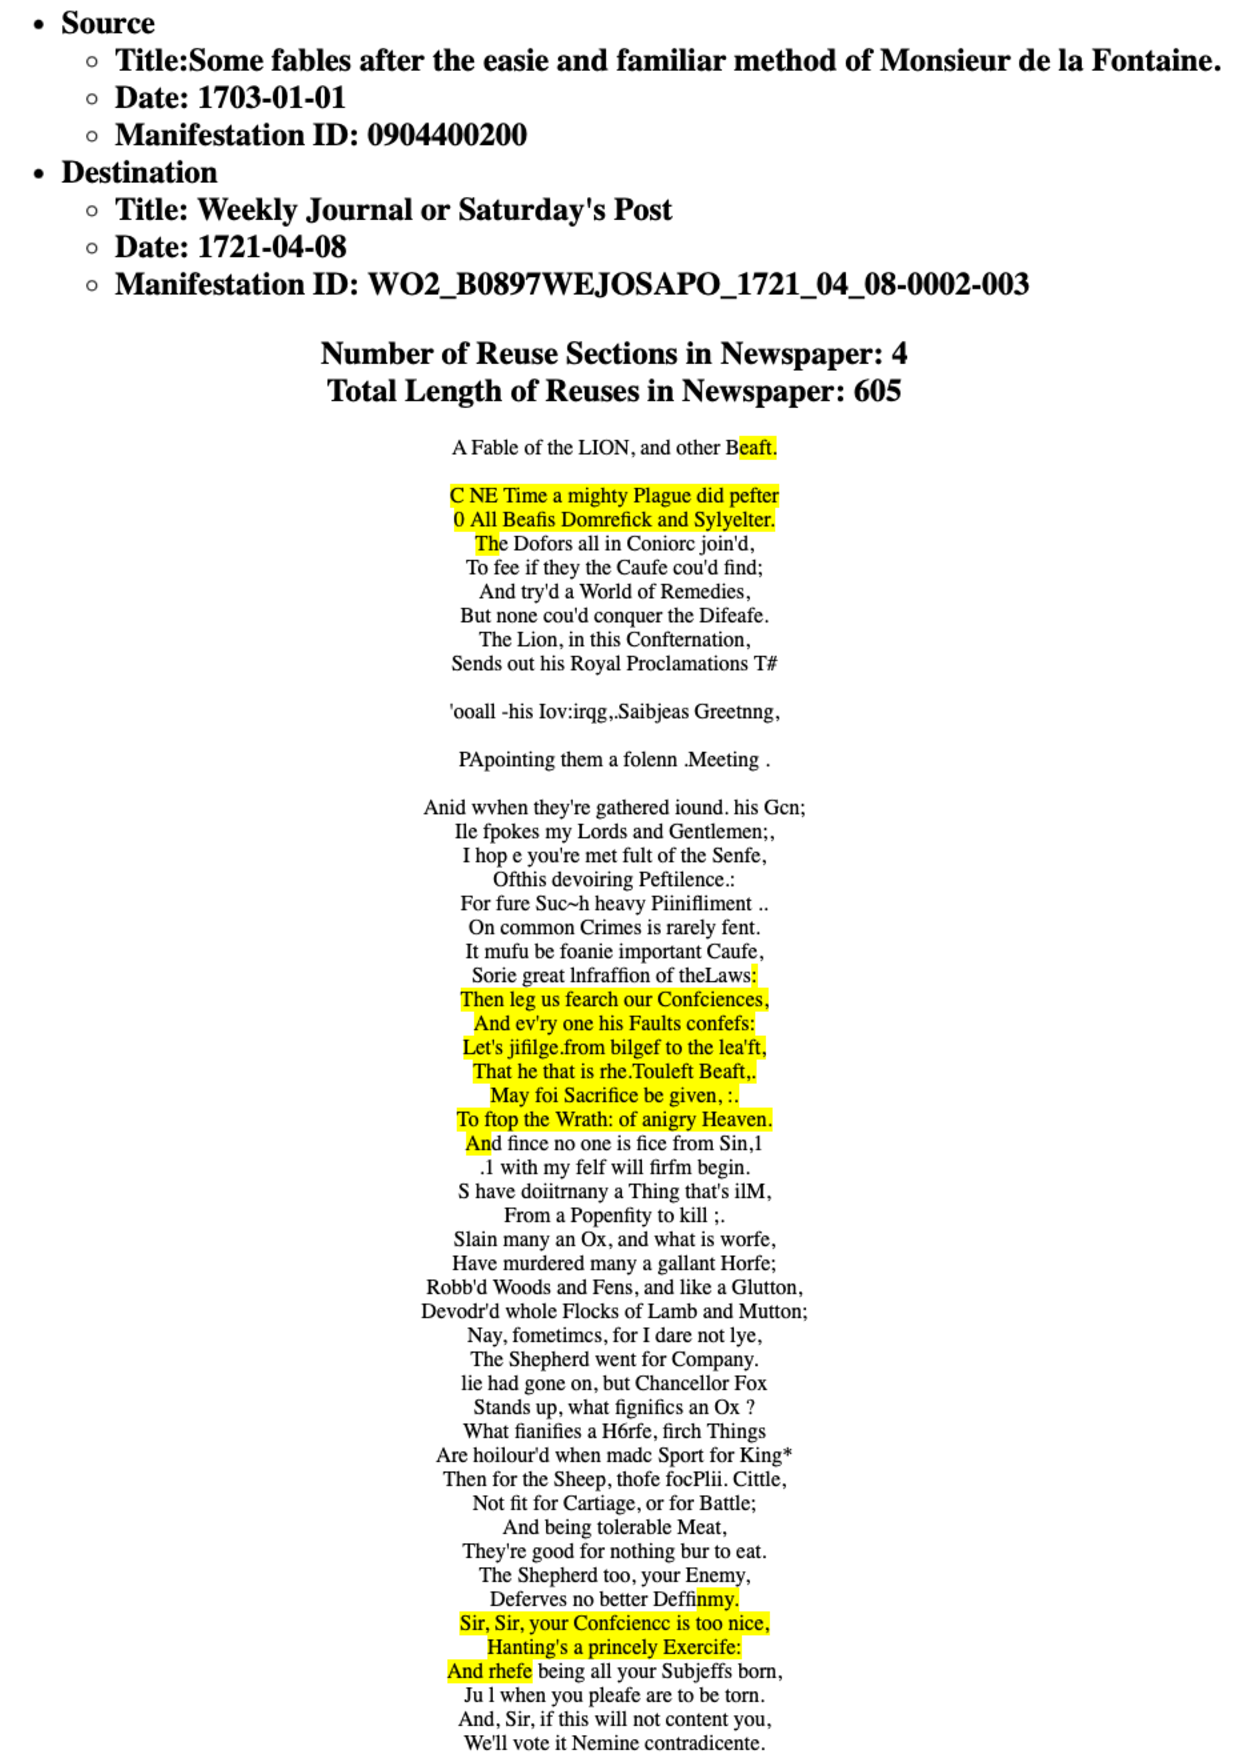
\includegraphics[width=\textwidth,clip,trim={0 24cm 0 0}]{images/newspaper_analysis.pdf}
%     \end{center}
%     \vspace{1cm}
%   \end{minipage}%
%   \begin{minipage}{0.5\textwidth}
%     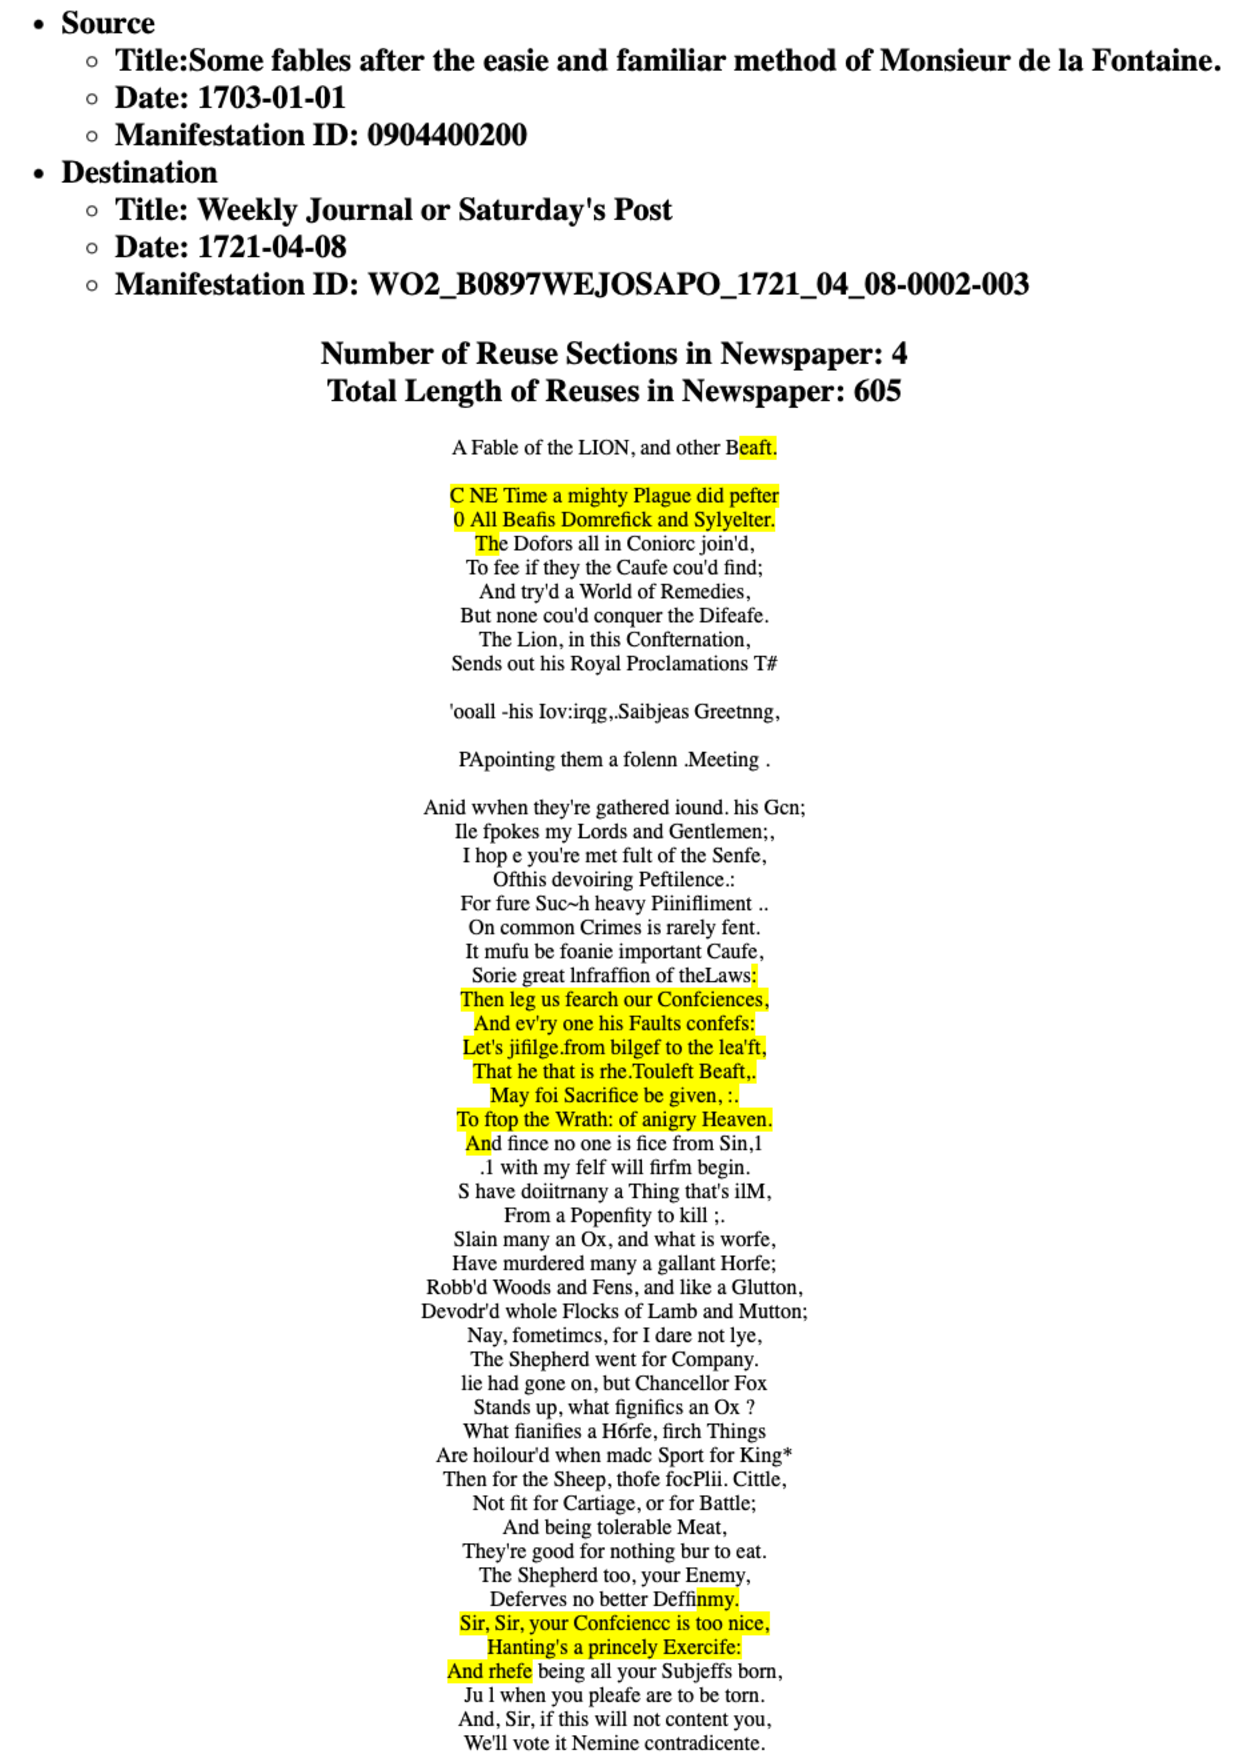
\includegraphics[keepaspectratio,height=\textheight,clip,trim={0 0 0 5.2cm}]{images/newspaper_analysis.pdf}
    
%   \end{minipage}

% \end{frame}


\subsection{Locke Quotes Task}

\begin{frame}
  \frametitle{Locke Quotes Task}
  % Top-$k$ Quotes Example Task:\\\\\noindent
  \begin{columns}
    
    \begin{column}{0.5\textwidth}
      {\textbf{Document}: John Locke: An essay concerning humane understanding\\}
      {\textbf{Quote Length}: 150 -- 200 characters\\}
      {\textbf{Quote Metric}: Number of reuses in works of different authors\\}
      {\textbf{Quantity}: Top $k$ quotes\\}
    \end{column}
    \begin{column}{0.5\textwidth}
      Steps:
      \begin{enumerate}
        \item Find clusters where source piece belongs to \textbf{Document} and is of \textbf{Length}
        \item In each cluster find all destination pieces, their authors and filter out John Locke
        \item Count number of unique destination works for each source piece (\textbf{Metric})
        \item Return Top-$k$ source pieces as quotes (\textbf{Quantity})
      \end{enumerate}
    \end{column}
  \end{columns}
\end{frame}
   

\begin{frame}[fragile]
  \frametitle{Complex Query}
  \begin{minted}[fontsize=\tiny,linenos=true]{sql}
WITH filtered_clusters AS (
    SELECT cluster_id, dp.*  FROM edition_ids
    INNER JOIN textreuse_edition_mapping USING(edition_id_i)
    INNER JOIN defrag_pieces dp USING(trs_id)
    INNER JOIN earliest_work_and_pieces_by_cluster USING(piece_id)
    WHERE edition_id = :estc_id AND dp.trs_end - dp.trs_start BETWEEN 150 AND 200
),query_authors AS (
	SELECT DISTINCT actor_id_i 
	FROM edition_authors 
	INNER JOIN edition_ids USING(edition_id_i)
	WHERE edition_id = :estc_id AND actor_id_i IS NOT NULL
), cluster_stats AS (
	SELECT cluster_id,COUNT(DISTINCT work_id_i) as n_works FROM filtered_clusters
	INNER JOIN non_source_pieces_tmp nsp USING (cluster_id)
	INNER JOIN defrag_pieces dp ON nsp.piece_id = dp.piece_id
	INNER JOIN textreuse_edition_mapping tem ON tem.trs_id = dp.trs_id
	INNER JOIN textreuse_work_mapping twm ON twm.trs_id = dp.trs_id
	INNER JOIN edition_authors USING(edition_id_i)
	LEFT JOIN query_authors qa USING(actor_id_i)
	WHERE qa.actor_id_i IS NULL 
	GROUP  BY cluster_id
),results AS (
	SELECT *,trs_end-trs_start AS piece_length FROM cluster_stats
	INNER JOIN filtered_clusters fc USING (cluster_id))
SELECT * FROM results
ORDER BY n_works DESC,piece_length DESC
LIMIT 100 
  \end{minted}
\end{frame}


\begin{frame}[fragile]
  \frametitle{Task Specific Data}
    
    \begin{center}
      
      \begin{tikzpicture}
        \tikzset{
          table/.style={
            rectangle split, 
            rectangle split parts=#1+1, 
            rectangle split part fill={gray!50,white},
            rectangle split draw splits=false,
            draw, 
            align=center,
            rounded corners,
            inner sep=0.5mm,
            font=\small,
            },
            every label/.style={align=center}
            }
            \node[table=9, anchor=north west, label={Top Quotes Task Data}] at (0,0) (source-piece-metrics) { 
              {source\_piece\_statistics\_denorm} 
              \nodepart{two} {piece\_id} 
              \nodepart{three} {cluster\_id}
              \nodepart{four} {manifestation\_id} 
              \nodepart{five} {trs\_start} 
              \nodepart{six} {trs\_end} 
              \nodepart{seven} {piece\_length} 
              \nodepart{eight} {num\_reception\_edges} 
              \nodepart{nine} {num\_different\_work\_ids} 
              \nodepart{ten} {num\_work\_ids\_different\_authors} 
              };    

            \draw<2>[thick,red] (source-piece-metrics.text split west) rectangle (source-piece-metrics.four split east);  
            \node[right=1cm of source-piece-metrics.three east] {{\visible<2>{IDs}}};
            \draw<3>[thick,red] (source-piece-metrics.four split west) rectangle (source-piece-metrics.six split east);  
            \node[right=1cm of source-piece-metrics.five split east] {{\visible<3>{Offsets}}};
            \draw<4>[thick,red] (source-piece-metrics.six split west) rectangle (source-piece-metrics.south east);  
            \node[right=1cm of source-piece-metrics.eight split east] {{\visible<4>{Metrics}}};
            \end{tikzpicture}
            
          \end{center}
      \end{frame}


  % \begin{frame}
  %   \frametitle{Dagster Upstream Assets}
  %   {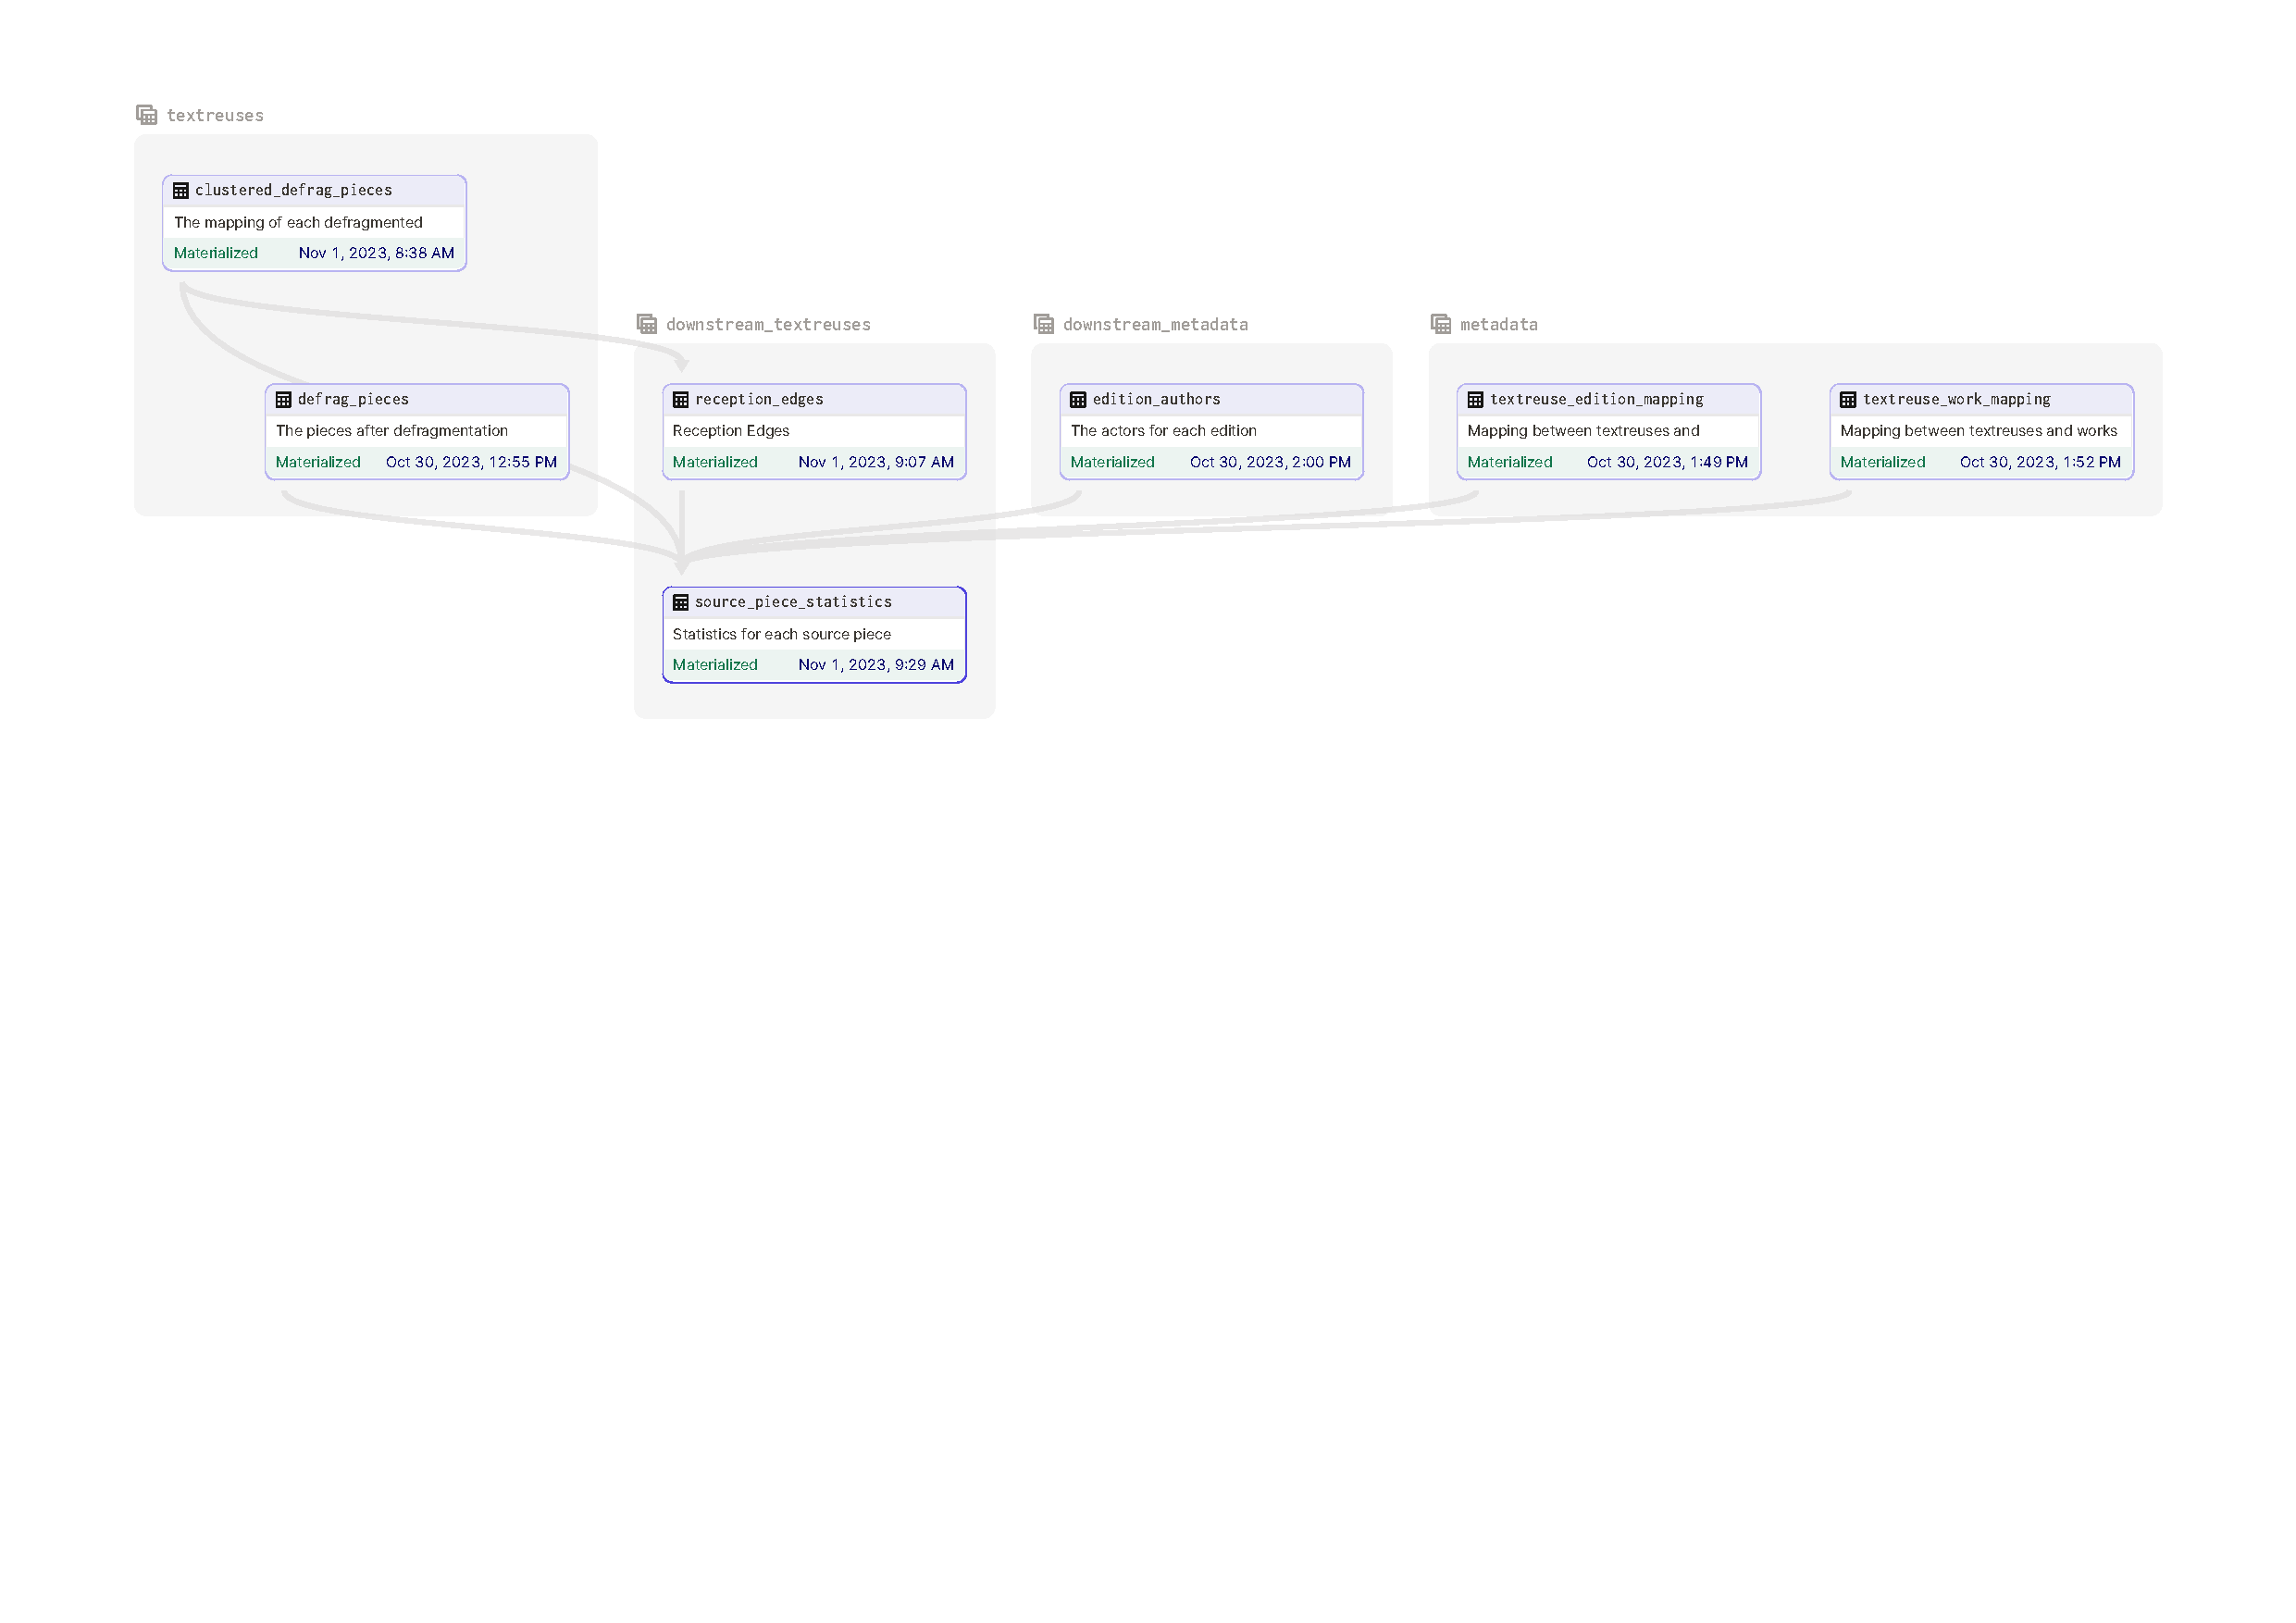
\includegraphics[width=\textwidth,clip,trim={ 1.5cm 15cm 2cm 2cm}]{images/Assets_source_piece_statistics.pdf}}
  % \end{frame}

  \begin{frame}[fragile]
      \frametitle{Simple Query}
  \begin{columns}
    \begin{column}{0.5\textwidth}   
      \begin{itemize}
        \item \textbf{Document}\tikzmark{doc}
        \item \textbf{Quote Length}\tikzmark{l}
        \item \textbf{Quote Metric}\tikzmark{metric}
        \item \textbf{Quantity}\tikzmark{num}
      \end{itemize}
    \end{column}
    \begin{column}{0.5\textwidth}
      \begin{minted}[escapeinside=||,fontfamily=tt,
        fontsize=\scriptsize,linenos=true,]{sql}
|\tikzmark{selectstart}|SELECT|\tikzmark{selectend}|
    piece_length as length, 
    num_work_ids_different_authors as metric,
    piece_text(ts.text,trs_start,trs_end) as text 
|\tikzmark{fromstart}|FROM|\tikzmark{fromend}|
    |\tikzmark{tablestart}|source_piece_statistics_denorm spsd|\tikzmark{tableend}|
    |\tikzmark{idsstart}|INNER JOIN textreuse_ids ti USING(trs_id)|\tikzmark{idsend}|
    INNER JOIN textreuse_sources ts USING(trs_id)
|\tikzmark{wherestart}|WHERE|\tikzmark{whereend}|
    |\tikzmark{docstart}|manifestation_id = "A48874"|\tikzmark{docend}|
    |\tikzmark{lstart}|AND piece_length BETWEEN 150 AND 200|\tikzmark{lend}|
    |\tikzmark{metricstart}|AND num_work_ids_different_authors >=20|\tikzmark{metricend}|
|\tikzmark{orderstart}|ORDER BY|\tikzmark{orderend}|
    num_work_ids_different_authors DESC,
    trs_start 
|\tikzmark{limitstart}|LIMIT 12|\tikzmark{limitend}|
    \end{minted}
    
\begin{tikzpicture}[remember picture,overlay]
  \fill[black,bg,opacity=0.6] ([yshift=+1ex]pic cs:selectstart) rectangle ([yshift=-0.5ex,xshift=\textwidth]pic cs:fromend);
  \fill[bg,opacity=0.6] ([yshift=-2ex]pic cs:fromstart) rectangle ([yshift=-0.5ex,xshift=\textwidth+2ex]pic cs:wherestart);
  \fill[bg,opacity=0.6] ([yshift=+1ex]pic cs:orderstart) rectangle ([yshift=+1ex,xshift=\textwidth]pic cs:limitstart);
  % \draw<2>[red] ([yshift=+1ex,xshift=-0.25ex]pic cs:tablestart) rectangle ([yshift=-0.5ex,xshift=+0.25ex]pic cs:tableend);
  % \draw<3>[red] ([yshift=+1ex,xshift=-0.25ex]pic cs:docstart) rectangle ([yshift=-0.5ex,xshift=+0.25ex]pic cs:docend);
  % \draw<4>[red] ([yshift=+1ex,xshift=-0.25ex]pic cs:lstart) rectangle ([yshift=-0.5ex,xshift=+0.25ex]pic cs:lend);
  % \draw<5>[red] ([yshift=+1ex,xshift=-0.25ex]pic cs:metricstart) rectangle ([yshift=-0.5ex,xshift=+0.25ex]pic cs:metricend);
  % \draw<6>[red] ([yshift=+1ex,xshift=-0.25ex]pic cs:limitstart) rectangle ([yshift=-0.5ex,xshift=+0.25ex]pic cs:limitend);
  \draw[red] ([yshift=+0.5ex]pic cs:doc) -- ([yshift=+0.5ex]pic cs:docstart);
  \draw[red] ([yshift=+0.5ex]pic cs:l) -- ([yshift=+0.5ex]pic cs:lstart);
  \draw[red] ([yshift=+0.5ex]pic cs:metric) -- ([yshift=+0.5ex]pic cs:metricstart);
  \draw[red] ([yshift=+0.5ex]pic cs:num) -- ([yshift=+0.5ex]pic cs:limitstart);
\end{tikzpicture}   
    \end{column}
  \end{columns}

\end{frame}

\begin{frame}[fragile]
  \frametitle{Query Results}
  % \vspace*{-0.5cm}
  \begin{table}[!ht]
    \tiny
    \centering
    \vspace*{-0.1cm}
    \begin{tabular}{|c|c|c|p{10cm}|}
    \hline
        Index & Length & Metric & Text \\ \hline
        \tikzmark{start}1 & 172 & 42 & "everal degrees of pleasure and pain, in all the things that environ and affect us*; and blended them together, in almost all that our Thoughts and Senses have to do with; t" \\ \hline
        2 & 185 & 42 & "n separating carefully *Ideas* one from another, wherein can be found the least difference, thereby to avoid being misled by Similitude, and by affinity to take one thing for another. T" \tikzmark{end2}\\ \hline
        3 & 173 & 40 & "rom the other. There are Fishes that have Wings, and are not Strangers to the airy Reg\color<3>{red}{ion: and there are some Birds, that are Inhabitants of the Water; whose Bloud is cold a}" \\ \hline
        \tikzmark{start4}4 & 192 & 39 & "l World, we see no Chasms, or Gaps. All quite down from us, the descent is by easie steps, and a continued series of Things, that in each remove, differ very little one from the other. There a" \\ \hline
        5 & 150 & 39 & ": Which if it be probable, we have reason then to be perswaded, that there are far more Species of Creatures above us, than there are beneath; we bein"\tikzmark{end5} \\ \hline
        6 & 194 & 37 & "\textcolor<3>{red}{ion: and there are some Birds, that are I\textcolor<4>{red}{nhabitants of the Water; whose Bloud is cold a}}\textcolor<4>{red}{s Fishes, and their Flesh in taste so near akin, that the Scrupulous are allow'd them on Fish-days. Ther}e a" \\ \hline
        \tikzmark{start7}7 & 171 & 37 & "e being, in degrees of Perfection, much more remote from the infinite Being of GOD, than we are from the lowest state of Being, and that which approaches nearest to nothin" \\ \hline
        8 & 191 & 36 & "hat the Species of Creatures should also, by gentle degrees, ascend upward from us towards his infinite Perfection, as we see they gradually descend from us downwards: Which if it be probable" \\ \hline
        9 & 165 & 34 & "en both: Amphibious Animals link the Terrestrial and Aquatique together; Seales live at Land and at Sea, and Porpoises have the warm Bloud and Entrails of an Hog, no" \\ \hline
        10 & 176 & 27 & "njoyments of the Creatures can afford us, might be led to seek it in the enjoyment of him, *with whom there is fulness of joy, and at whose right hand are pleasures for evermor"\tikzmark{end10} \\ \hline
        11 & 150 & 23 & "\textcolor<4>{red}{nhabitants of the Water; whose Bloud is cold as Fishes, and their Flesh in taste so near akin, that the Scrupulous are allow'd them on Fish-days. Ther}" \\ \hline%
        \tikzmark{start12}12 & 153 & 23 & "hey gradually descend from us downwards: Which if it be probable, we have reason then to be perswaded, that there are far more Species of Creatures above"\tikzmark{end} \\ \hline
    \end{tabular}
\end{table}
\begin{tikzpicture}[remember picture,overlay]
  \fill<2->[black,bg,opacity=0.85] ([yshift=+1ex,xshift=-5ex]pic cs:start) rectangle ([yshift=-0.4ex,xshift=\textwidth]pic cs:end2);
  \fill<2->[black,bg,opacity=0.85] ([yshift=+1ex,xshift=-5ex]pic cs:start4) rectangle ([yshift=-0.4ex,xshift=\textwidth]pic cs:end5);
  \fill<2->[black,bg,opacity=0.85] ([yshift=+1ex,xshift=-5ex]pic cs:start7) rectangle ([yshift=-0.4ex,xshift=\textwidth]pic cs:end10);
  \fill<2->[black,bg,opacity=0.85] ([yshift=+1ex,xshift=-5ex]pic cs:start12) rectangle ([yshift=-0.4ex,xshift=\textwidth]pic cs:end);
\end{tikzpicture} 

  

\end{frame}

% \begin{frame}
%   \frametitle{\href{https://www.receptionreader.com/d/A48874?from=1690&to=1800}{Reception Reader}}
%   \centering
%   {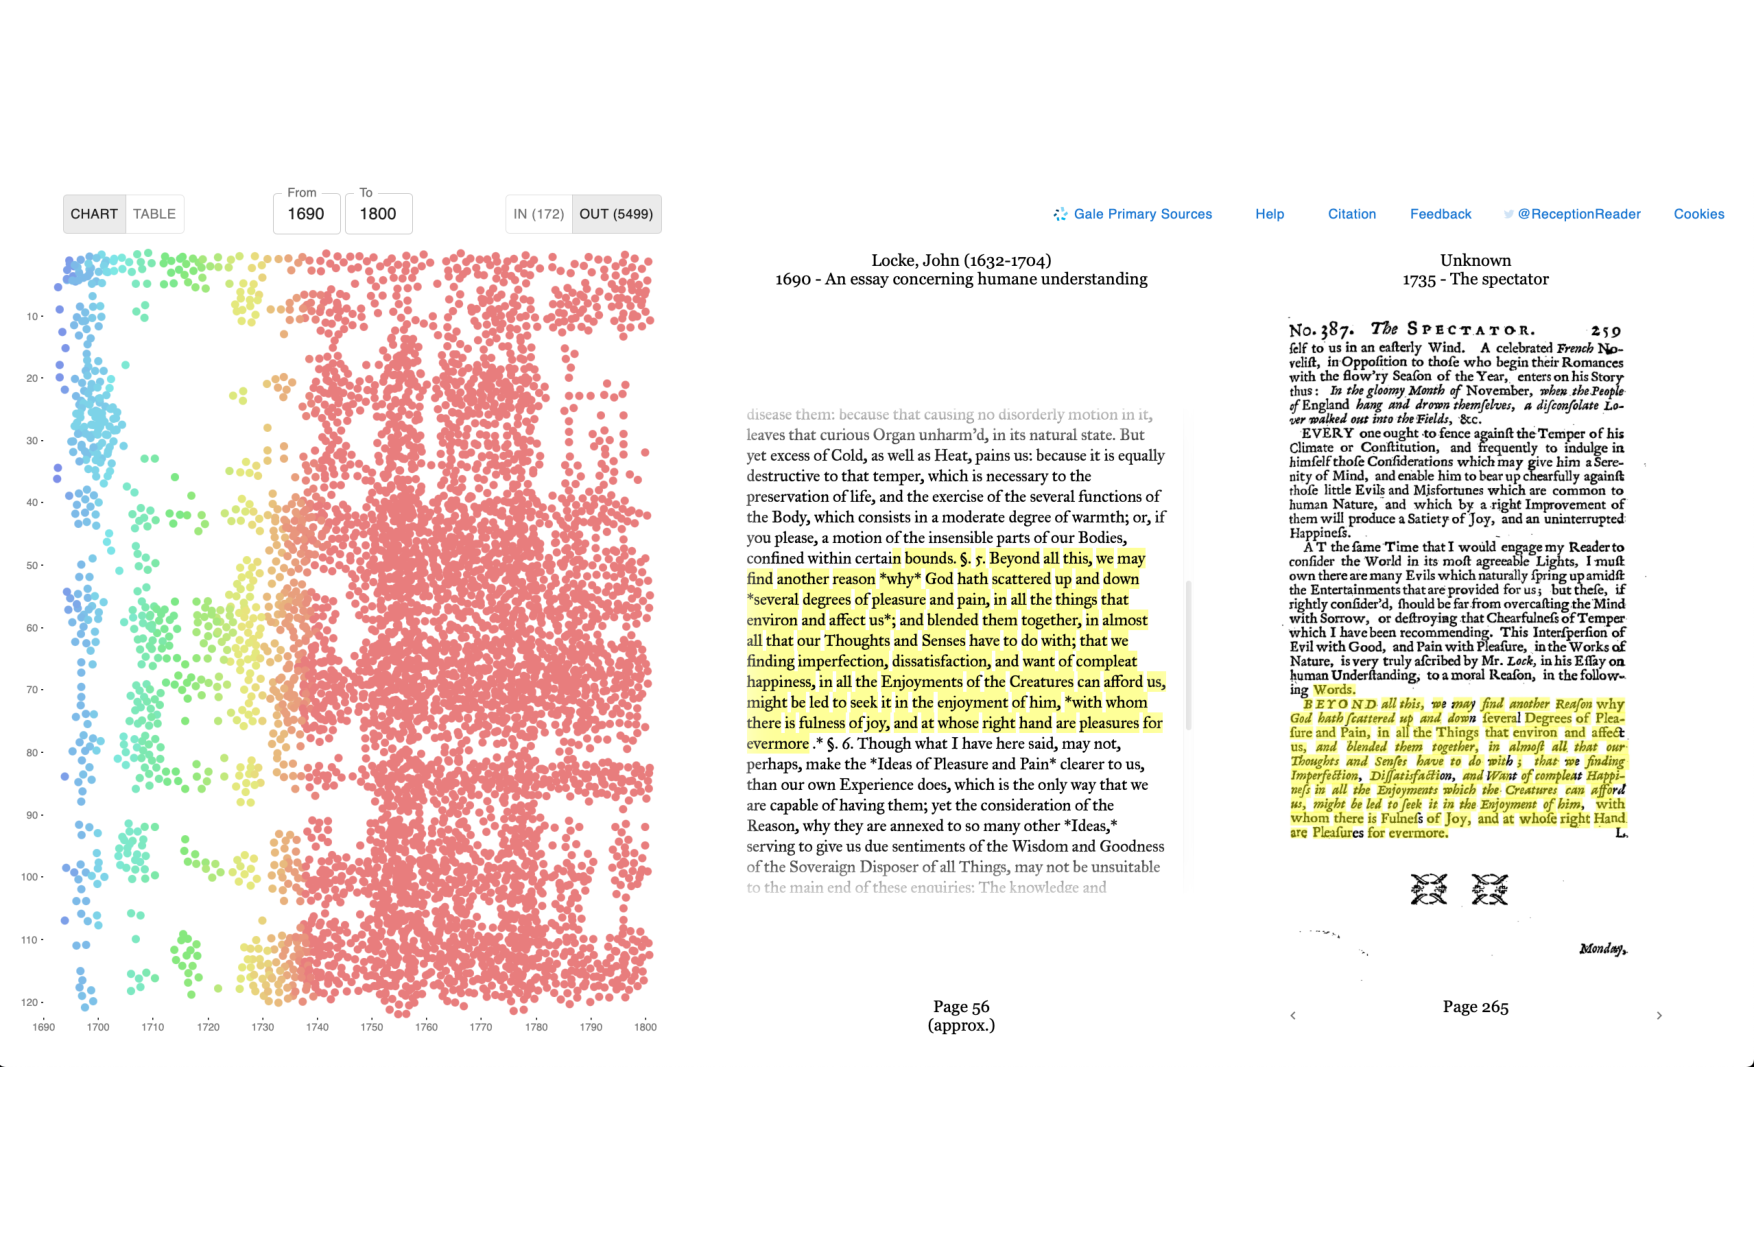
\includegraphics[clip,trim={0 3.5cm 0 3.5cm},keepaspectratio,height=0.8\textheight,width=\textwidth]{images/reception_reader.pdf}}
  

% \end{frame}


% \begin{frame}
%   \frametitle{Technology Stack}

%   \begin{enumerate}
%     \item Identifying lexical reuses
%     \begin{itemize}
%       \item High Performance Computing (HPC) cluster
%     \end{itemize}
%     \item ETL Stages
%     \begin{itemize}
%       \item Apache Spark cluster for distributed processing 
%       \item Dagster for asset management 
%       \item S3 buckets for bulk storage
%     \end{itemize}
%     \item Interfaces
%     \begin{itemize}
%       \item MariaDB (Aria and ColumnStore) Databases
%       \item Reception Reader
%     \end{itemize}
%   \end{enumerate}
% \end{frame}

\section{Semantic Text Reuses}

\subsection{Semantic Pipeline}
\begin{frame}
  \frametitle{Semantic Pipeline}
  \begin{tikzpicture}[remember picture, overlay]
    \node[anchor=north east] at (current page.north east) {\href{https://turkunlp.org}{
\includegraphics[width=0.23\linewidth]{images/turkunlp.png}}};
  \end{tikzpicture}
  \begin{columns}
    \begin{column}{0.5\textwidth}
      \begin{enumerate}
        \item Sentence Transformers
        \begin{itemize}
          \item Sentence to vector embedding
          \item<2-> Semantically meaningful embeddings
          \item<3-> Comparing embeddings for similarity
        \end{itemize}
        \item<4-> FAISS (\underline{\textbf{F}}acebook \underline{\textbf{AI}} \underline{\textbf{S}}imilarity \underline{\textbf{S}}earch) 
        \begin{itemize}
          \item<5-> Inverted File Index
          \item<7-> Product Quantization
        \end{itemize}
        \item<8-> Multilingual semantic search
        \begin{itemize}
          \item Teacher: English Sentence BERT
          \item Student: Multilingual BERT
          \item Result: Multilingual Sentence BERT
        \end{itemize}
      \end{enumerate}
    \end{column}
    \begin{column}{0.5\textwidth}
      \begin{center}
        \only<1>{
          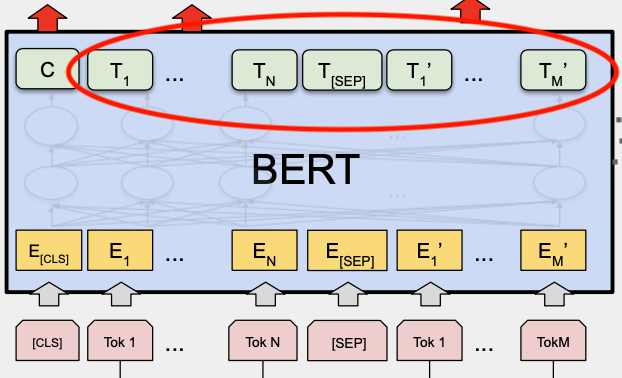
\includegraphics[width=0.8\textwidth]{images/bert.png}\\
          \href{https://arxiv.org/pdf/1810.04805}{\tiny BERT: Pre-training of Deep Bidirectional Transformers for Language Understanding}
        }   
        \only<2>{
          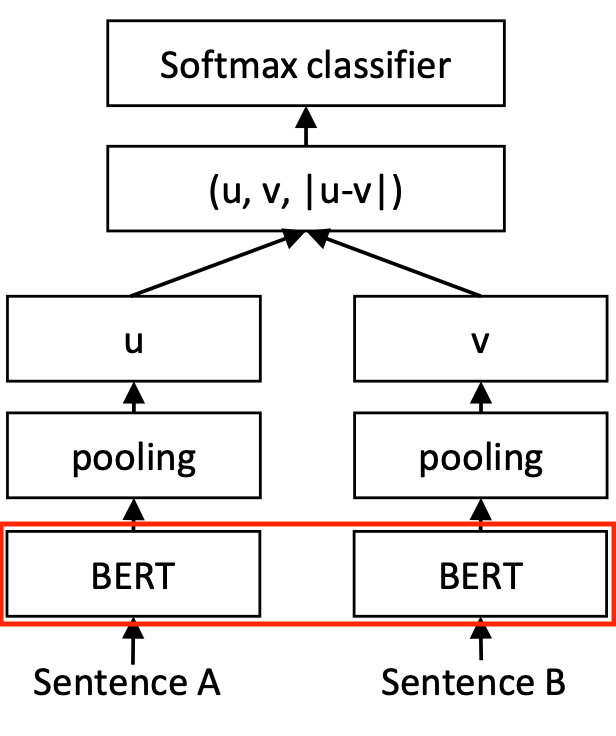
\includegraphics[width=0.6\textwidth]{images/sbert_finetuning.png}\\
          \href{https://arxiv.org/pdf/1908.10084}{\tiny Sentence-BERT: Sentence Embeddings using Siamese BERT-Networks}
          }
        \only<3>{
          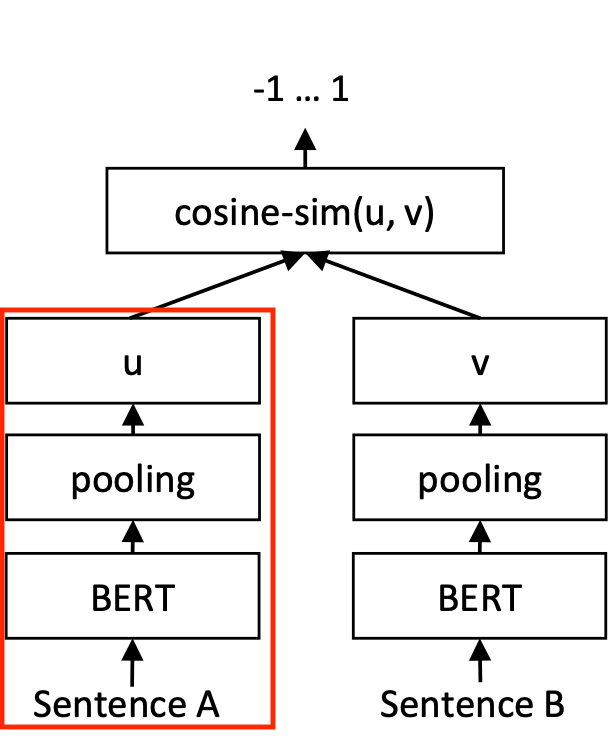
\includegraphics[width=0.6\textwidth]{images/sbert_inference.png}\\
          \href{https://arxiv.org/pdf/1908.10084}{\tiny Sentence-BERT: Sentence Embeddings using Siamese BERT-Networks}
          }
        \only<5>{
          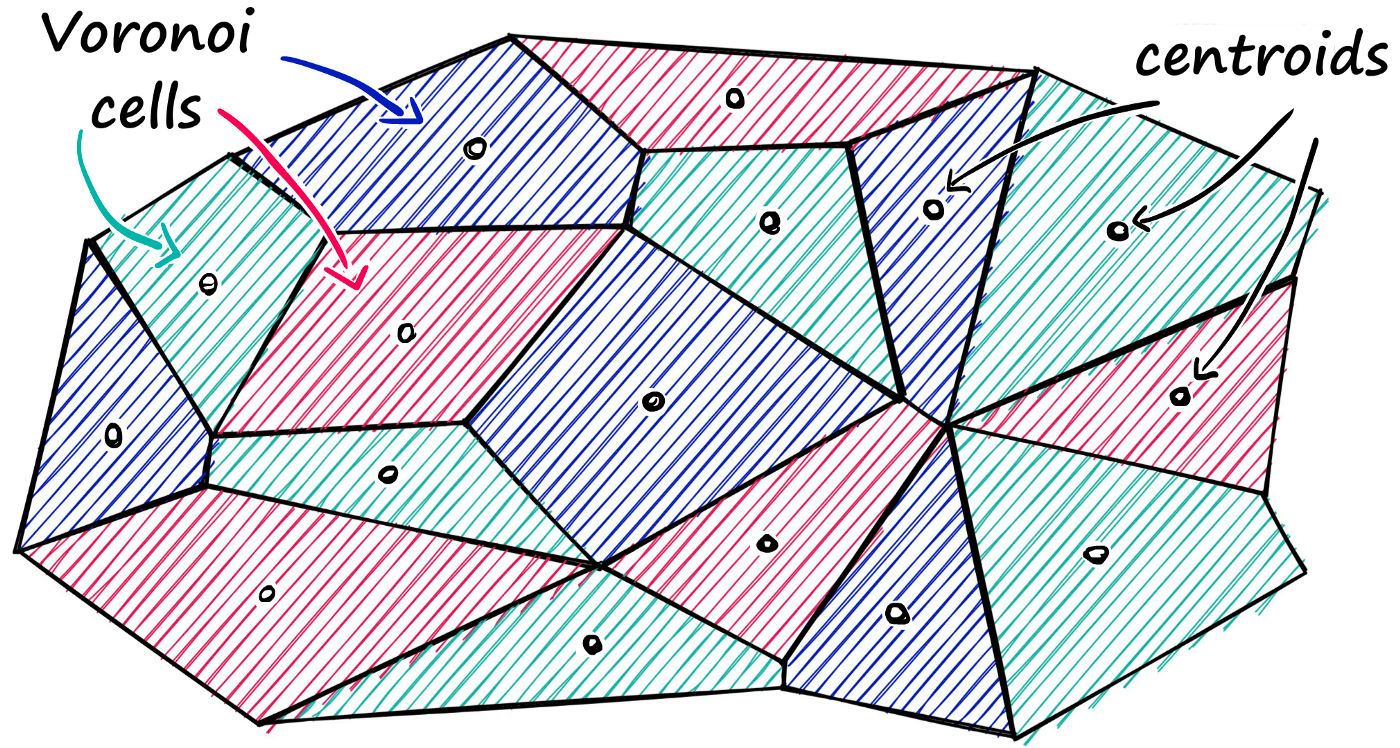
\includegraphics[width=\textwidth]{images/ivf_diagram.png}\\
          \href{https://www.pinecone.io/learn/series/faiss/faiss-tutorial/}{\tiny image source: pinecone.io FAISS-tutorial}
          }
        \only<6>{
          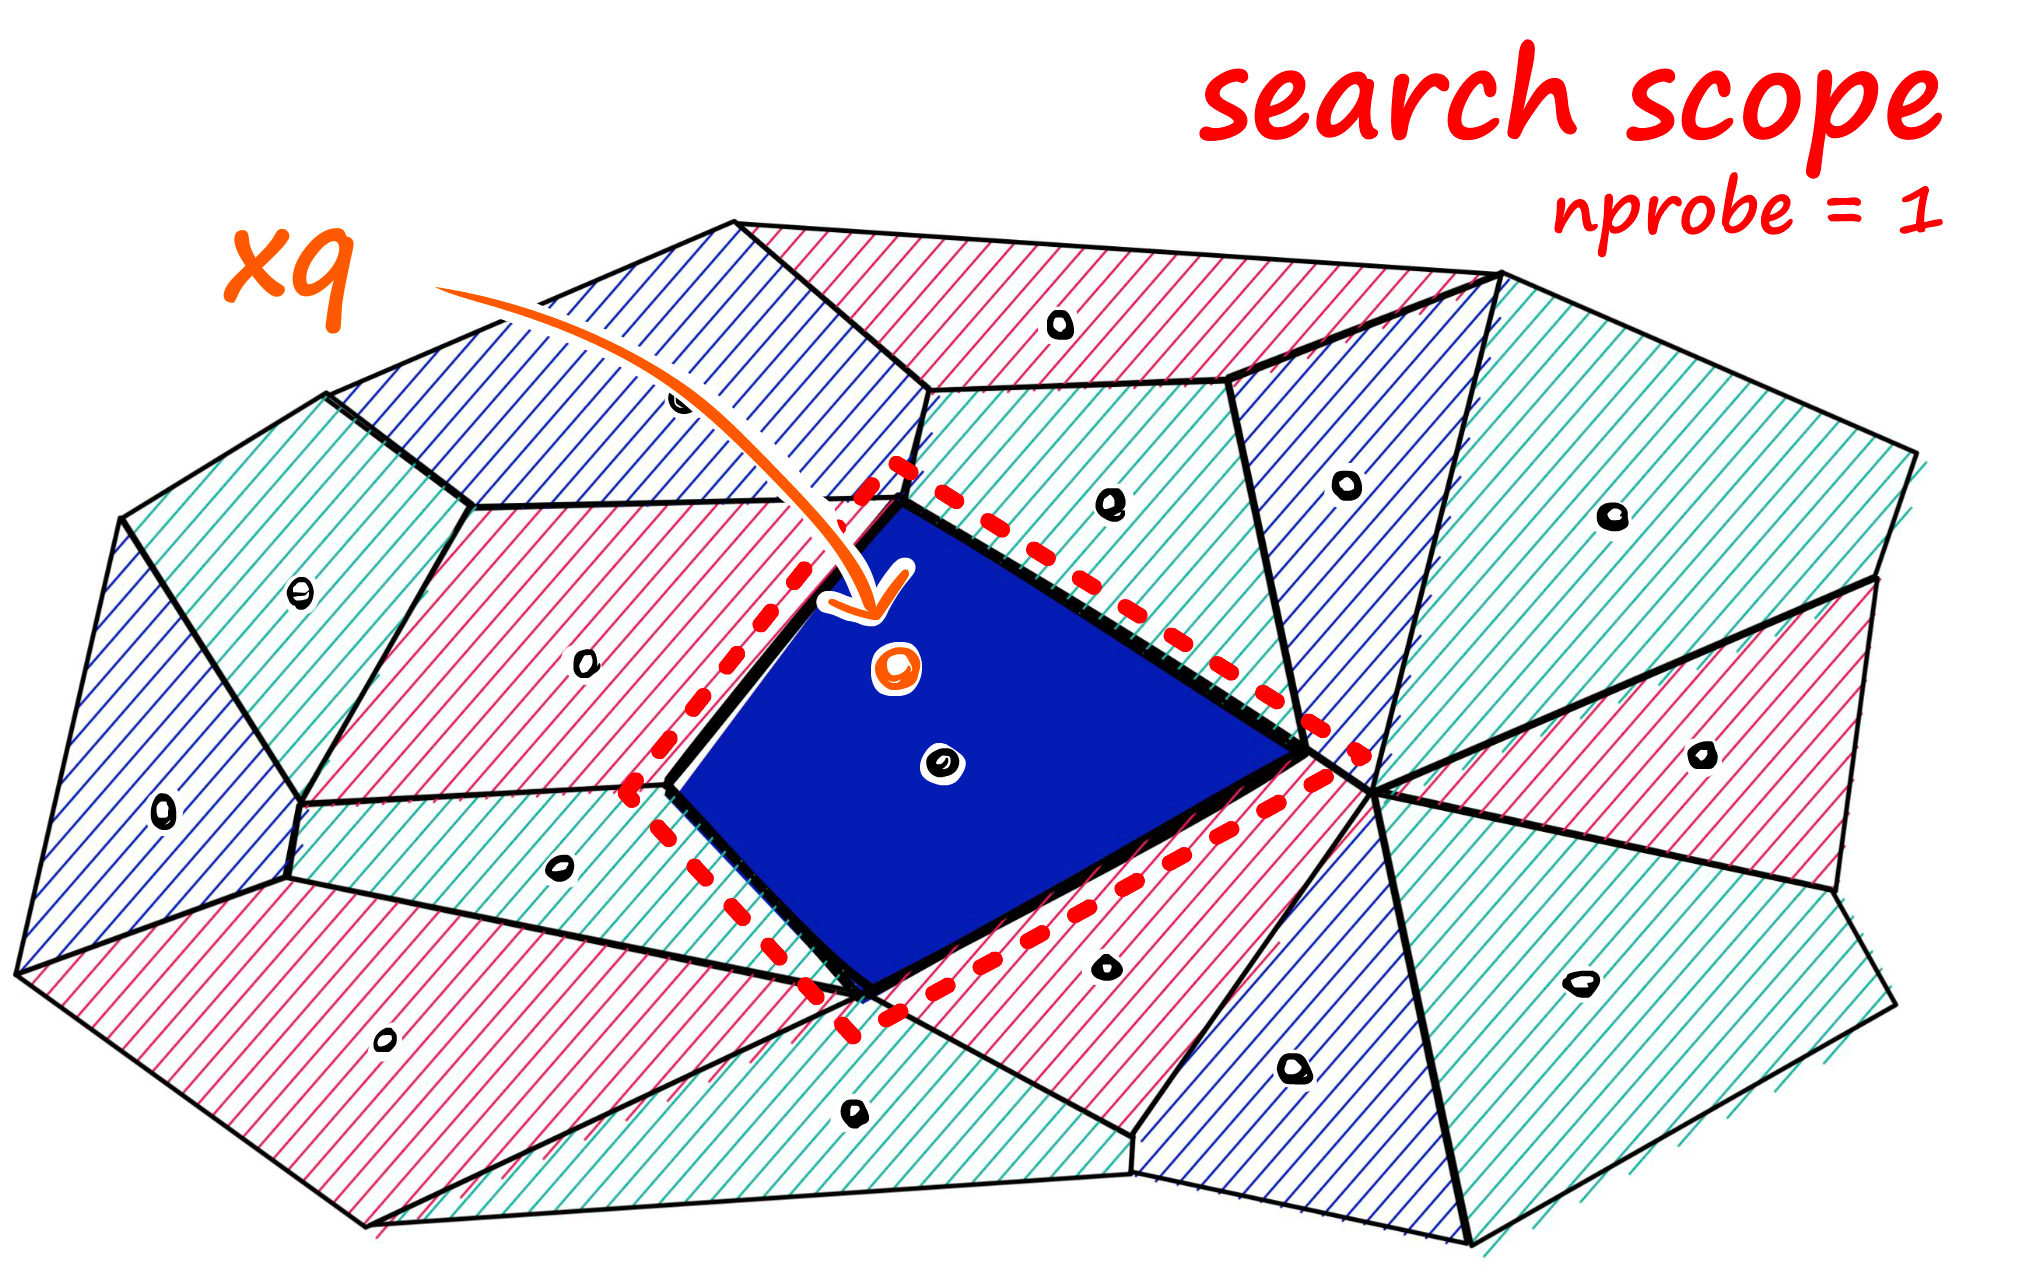
\includegraphics[width=\textwidth]{images/ivf_search.png}\\
          \href{https://www.pinecone.io/learn/series/faiss/faiss-tutorial/}{\tiny image source: pinecone.io FAISS-tutorial}
          }
        \only<7>{
          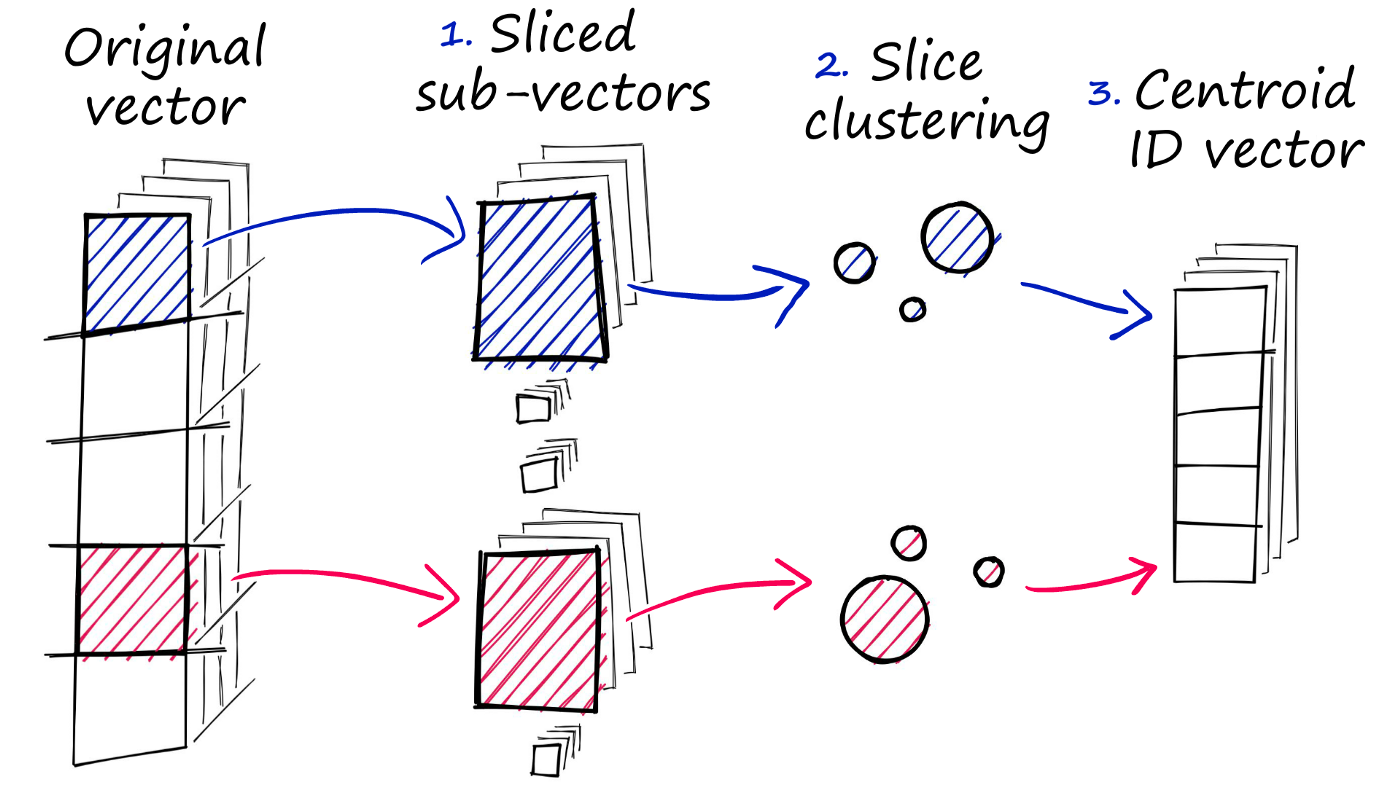
\includegraphics[width=\textwidth]{images/pq.png}\\
          \href{https://www.pinecone.io/learn/series/faiss/faiss-tutorial/}{\tiny image source: pinecone.io FAISS-tutorial}
          }
          \only<8>{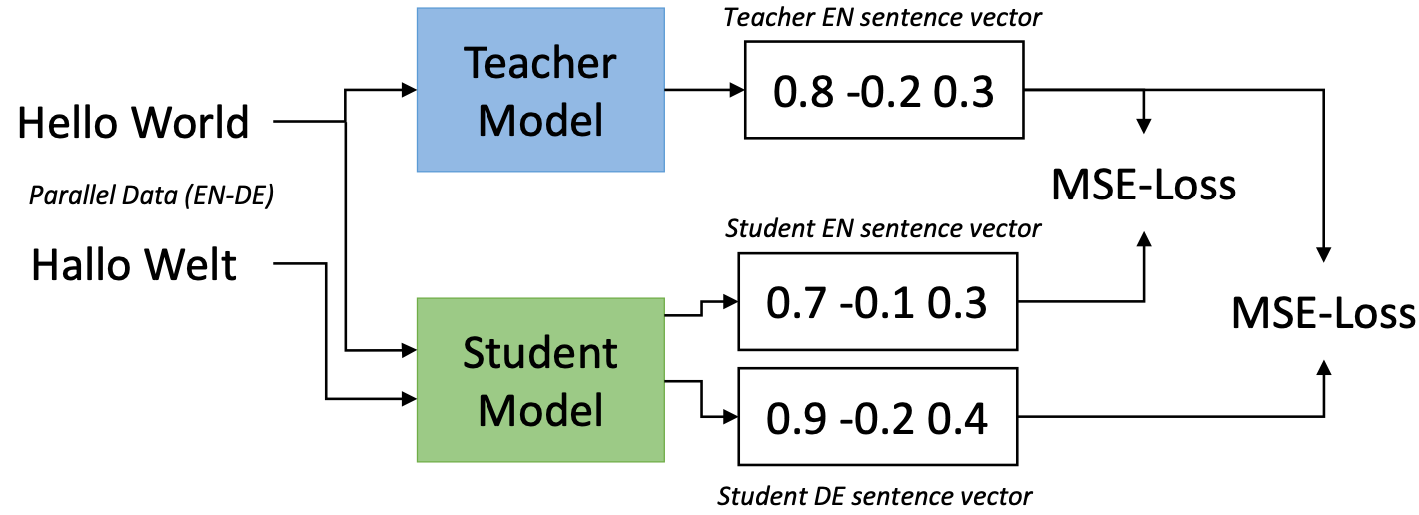
\includegraphics[width=\textwidth]{images/multilingual_training.png}\\
          \href{https://aclanthology.org/2020.emnlp-main.365.pdf}{\tiny Making Monolingual Sentence Embeddings Multilingual using Knowledge Distillation}
          }
        \end{center}
    \end{column}
  \end{columns}
  \end{frame}


\begin{frame}
  \frametitle{Interface}
  \begin{tikzpicture}[remember picture, overlay]
    \node[anchor=north east] at (current page.north east) {\href{https://turkunlp.org}{
\includegraphics[width=0.1\linewidth]{images/semantic_sim_qr.png}}};
  \end{tikzpicture}
  \vspace*{-0.1cm}
  \begin{columns}
  \begin{column}{0.5\textwidth}
      \centering
      \small English Query
      {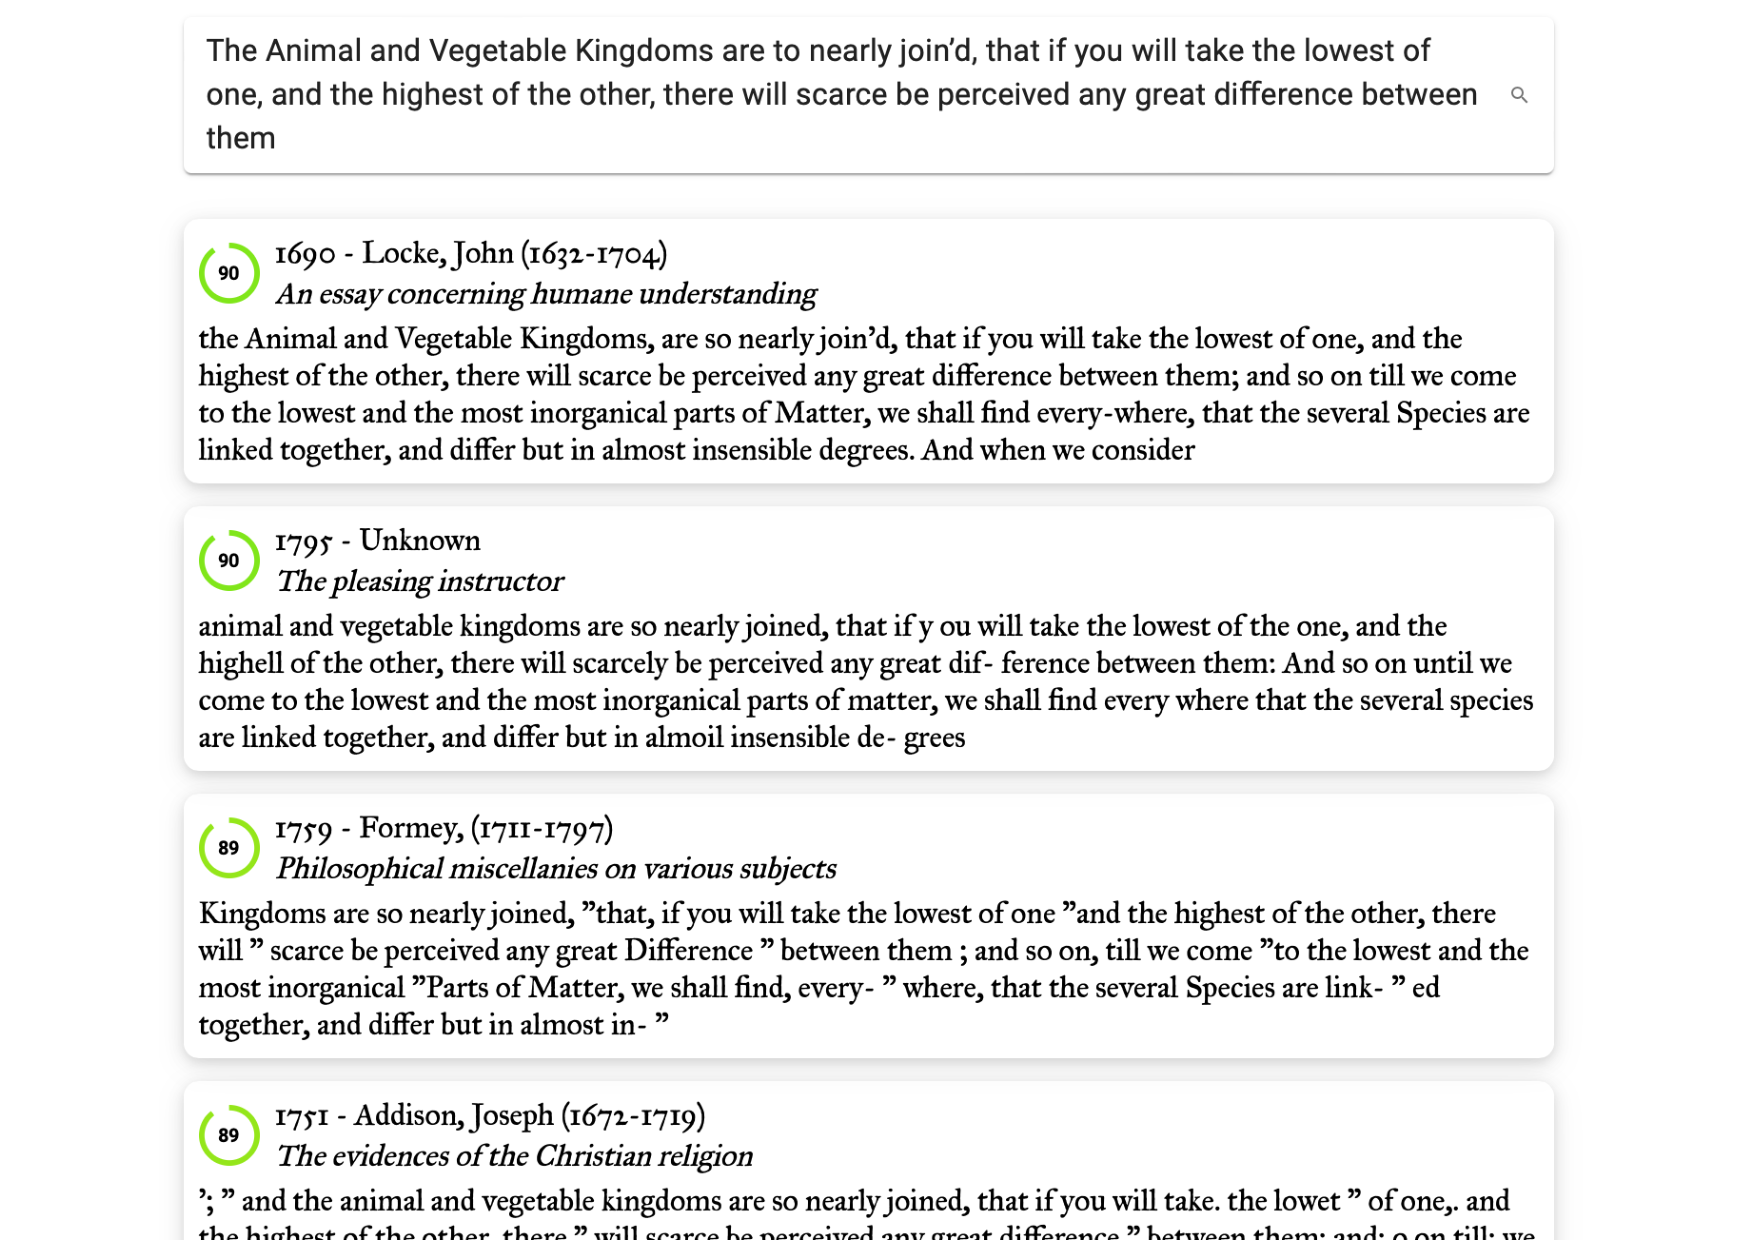
\includegraphics[width=\textwidth,height=\textheight,keepaspectratio,clip,trim={2.5cm 0 2.5cm 0}]{images/semantic_english.pdf}}
    \end{column}
  \begin{column}{0.5\textwidth}
      \centering
      \only<2>{
      {\small French Query}
      {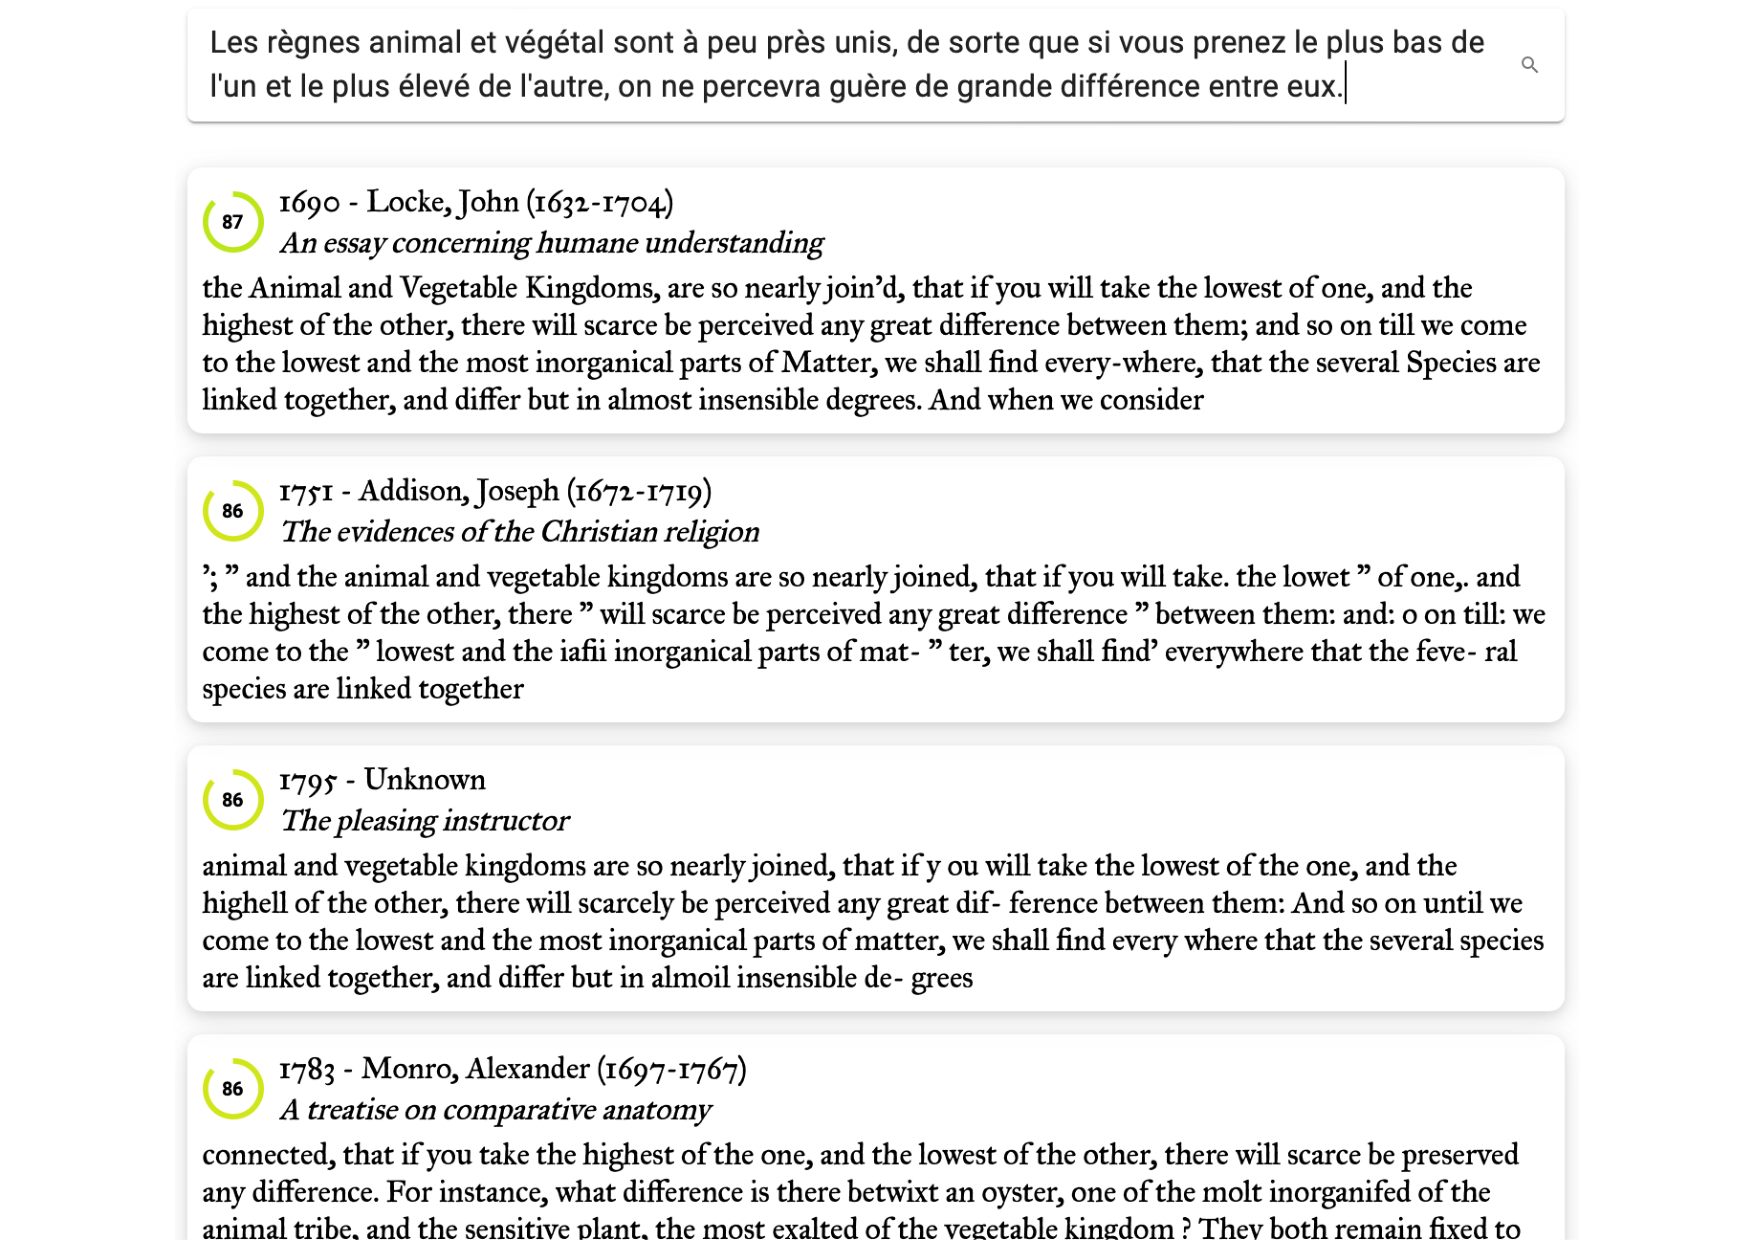
\includegraphics[width=\textwidth,,height=\textheight,keepaspectratio,clip,trim={2.5cm 0 2.5cm 0}]{images/semantic_french.pdf}}}
      \only<3>{
      {\small Spanish Query}
      {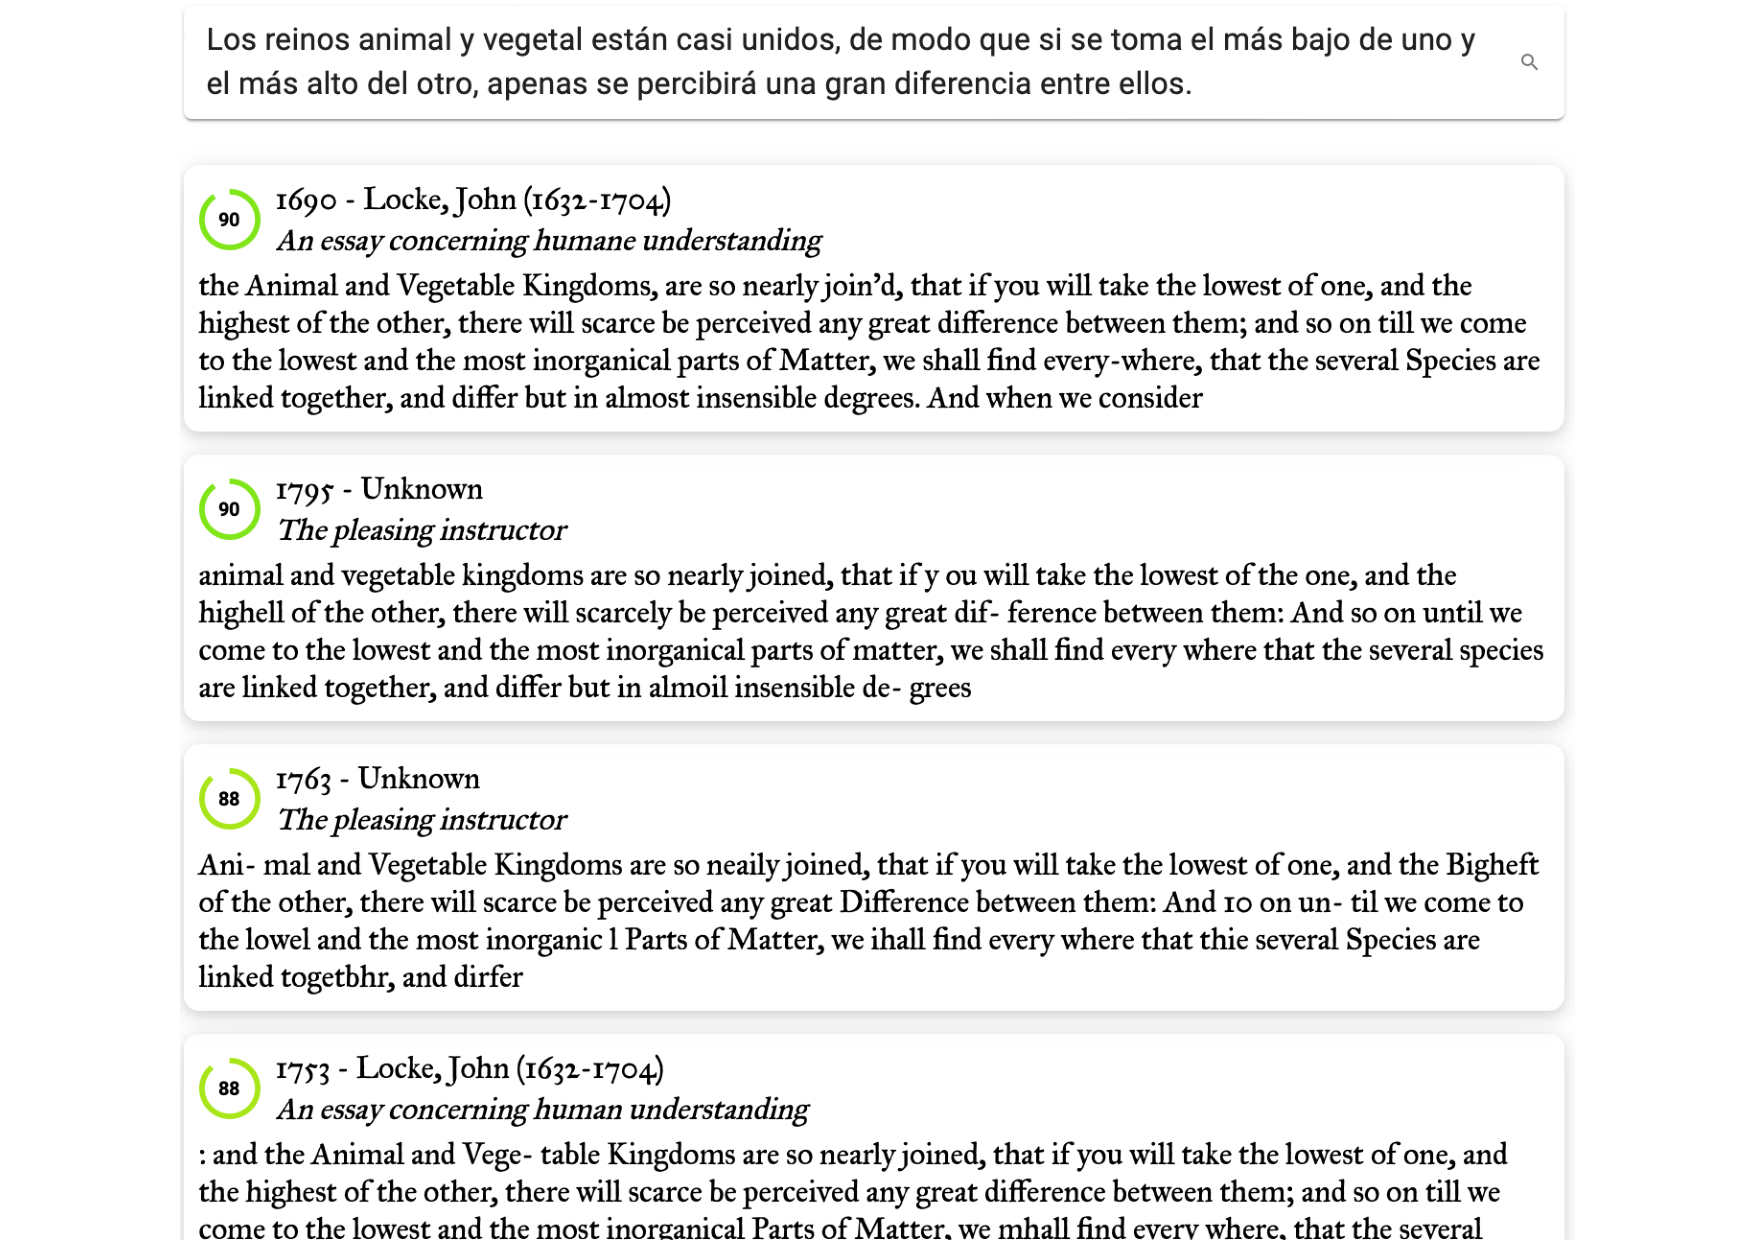
\includegraphics[width=\textwidth,,height=\textheight,keepaspectratio,clip,trim={2.5cm 0 2.5cm 0}]{images/semantic_spanish.pdf}}}
      \only<4>{
      {\small Tamil Query}
      {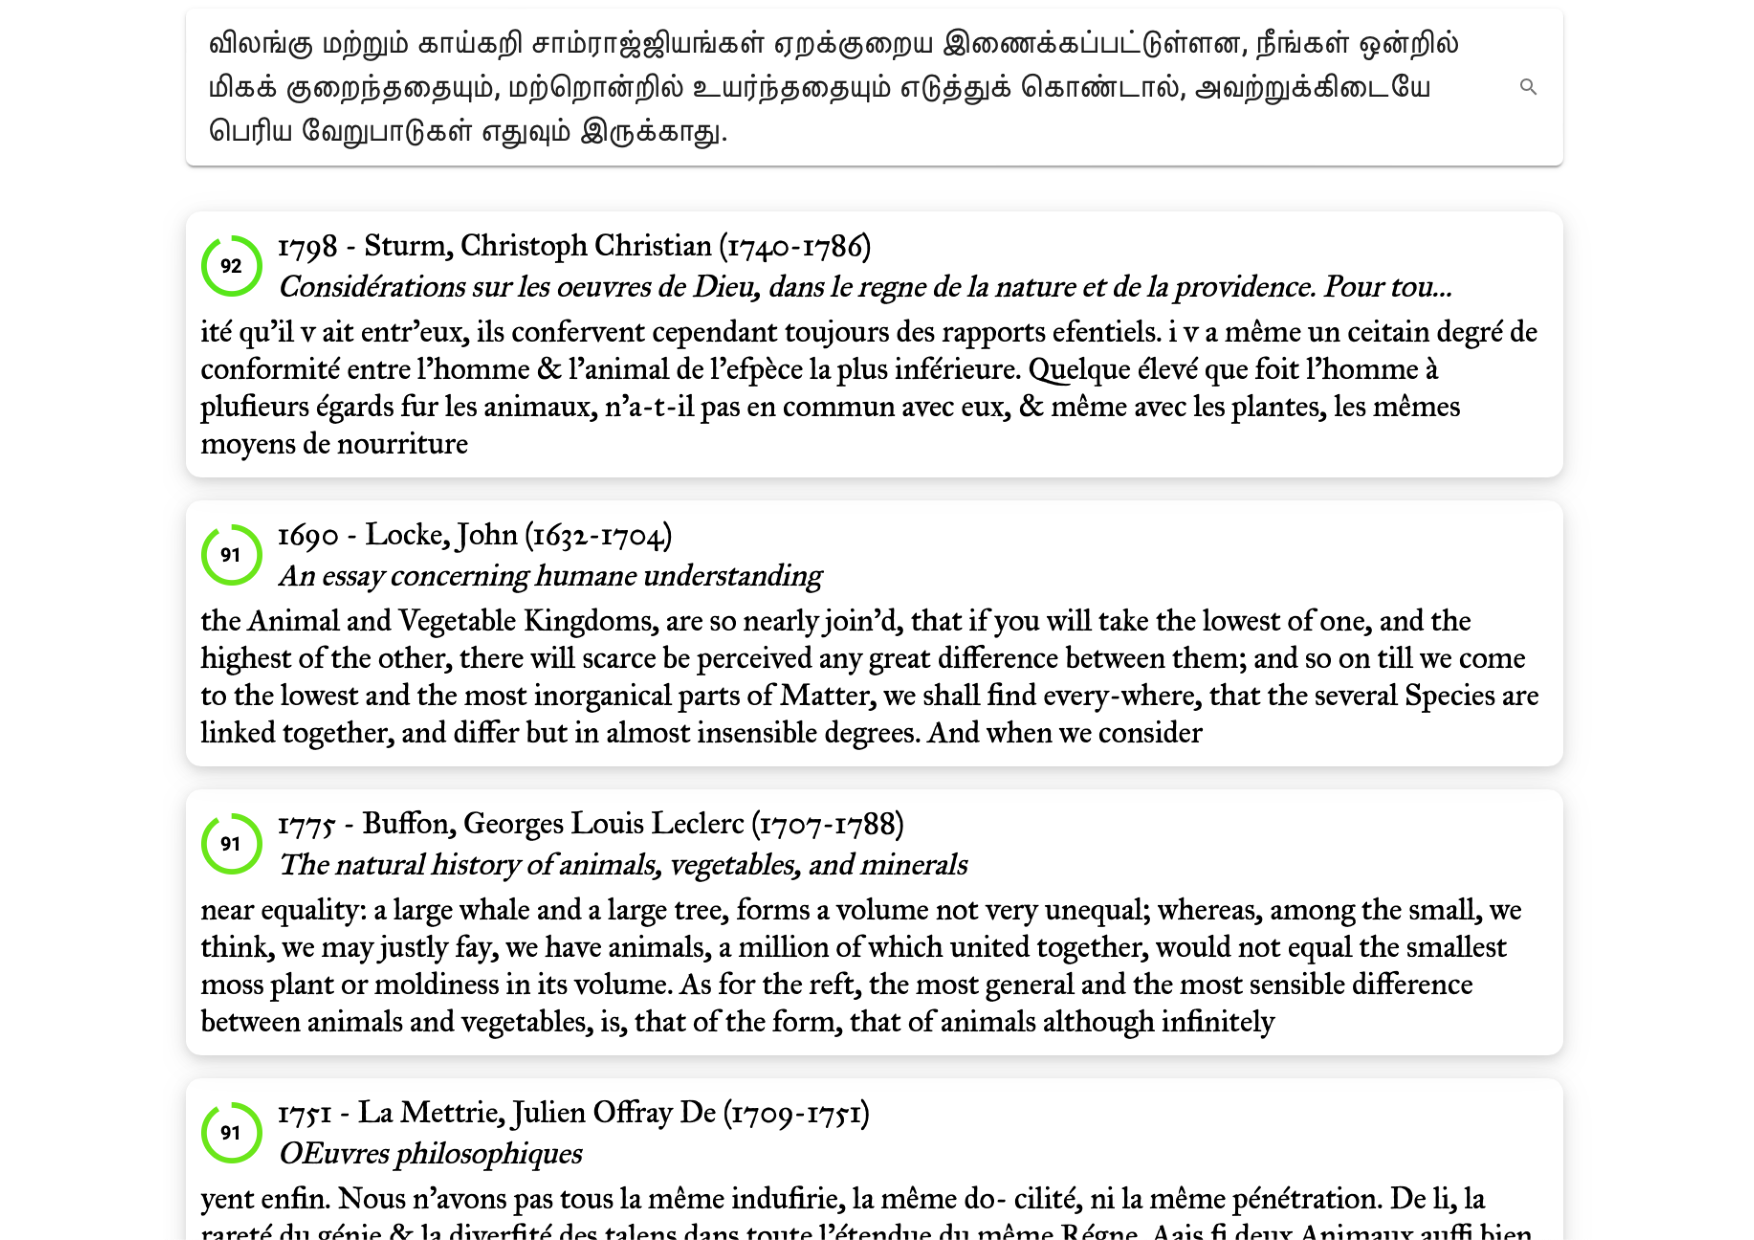
\includegraphics[width=\textwidth,,height=\textheight,keepaspectratio,clip,trim={2.5cm 0 2.5cm 0}]{images/semantic_tamil.pdf}}}
  \end{column}
  \end{columns}
\end{frame}

% \subsection{Sentence Transformer}

% \begin{frame}
%   \frametitle{Sentence Transformers}
%   \begin{tikzpicture}[remember picture, overlay]
%     \node[anchor=north east] at (current page.north east) {\href{https://turkunlp.org}{
\includegraphics[width=0.23\linewidth]{images/turkunlp.png}}};
%   \end{tikzpicture}
  

% \end{frame}


% \subsection{FAISS}

% \begin{frame}
%   \frametitle{FAISS}
%   \begin{tikzpicture}[remember picture, overlay]
%     \node[anchor=north east] at (current page.north east) {\href{https://turkunlp.org}{
\includegraphics[width=0.23\linewidth]{images/turkunlp.png}}};
%   \end{tikzpicture}
%   \begin{minipage}{0.5\textwidth}
%     Similarity metric: Cosine Similarity
%     \begin{enumerate}
%       \item<2-> Inverted File Index
%       \begin{itemize}
%         \item Partition space through clustering
%         \item<3-> Search in the closest cell for query
%       \end{itemize}
%       \item<4-> Product Quantization
%       \begin{itemize}
%         \item Chunk vectors into sub-vectors 
%         \item Find centroids in each chunk
%         \item Replace sub-vector with the closest centroid ID 
%       \end{itemize}  
%     \end{enumerate}
%   \end{minipage}%
%   \begin{minipage}{0.5\textwidth}
%     \begin{center}  
%       \only<2>{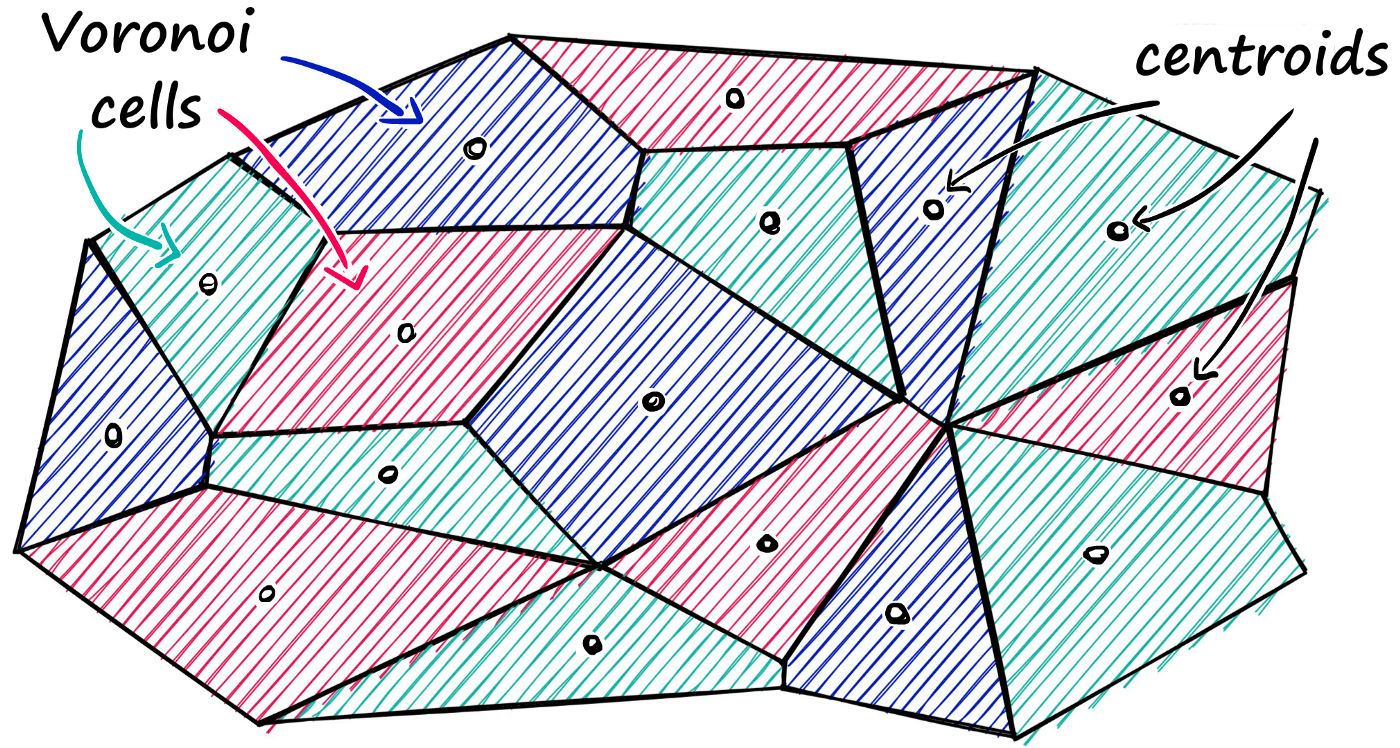
\includegraphics[width=\textwidth]{images/ivf_diagram.png}}
%       \only<3>{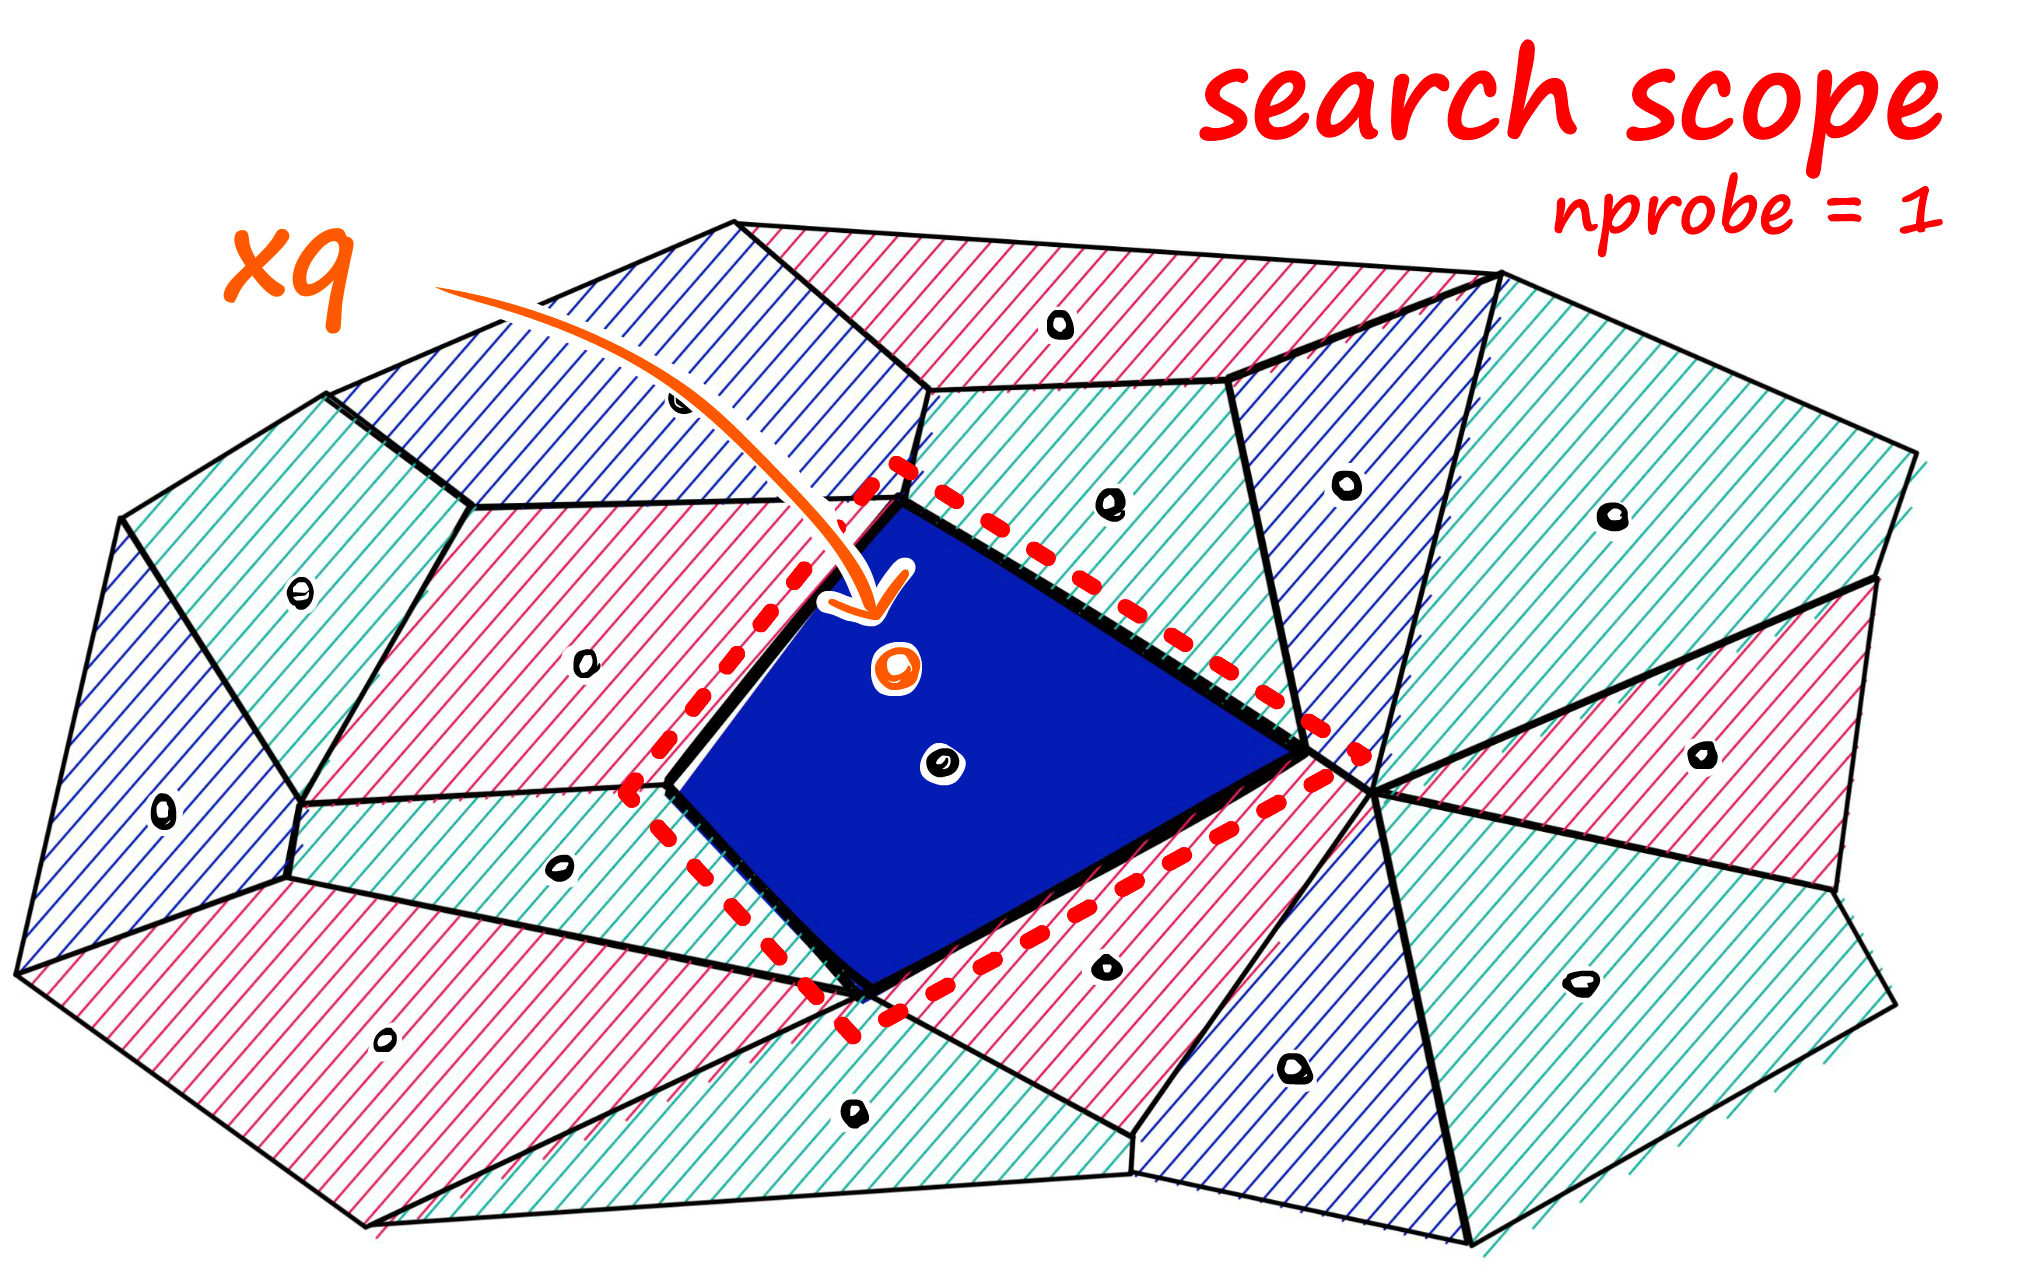
\includegraphics[width=\textwidth]{images/ivf_search.png}}
%       \only<4>{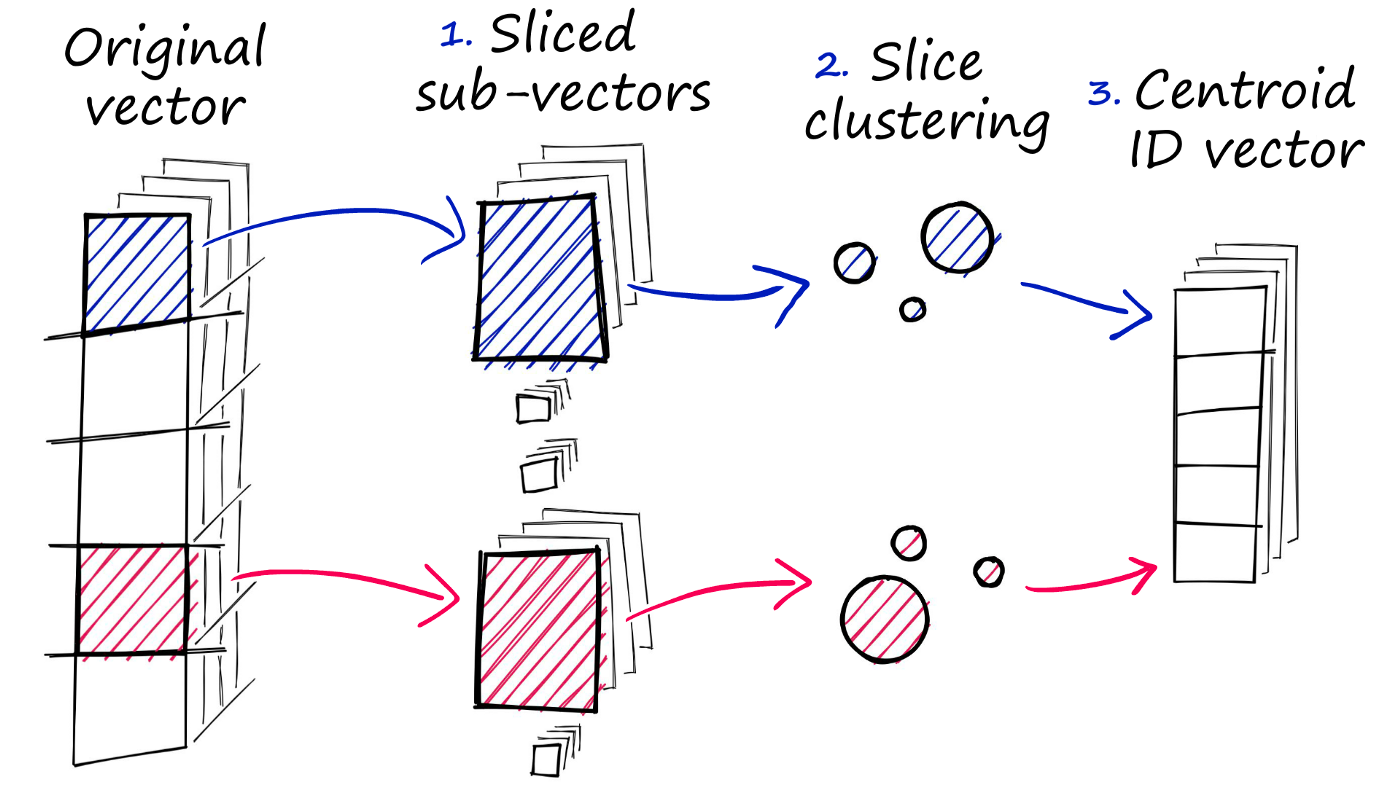
\includegraphics[width=\textwidth]{images/pq.png}}
%       \only<2->{\href{https://www.pinecone.io/learn/series/faiss/faiss-tutorial/}{\tiny image source: pinecone.io FAISS-tutorial}}
%     \end{center}
%     \end{minipage}
% \end{frame}


\subsection{Locke Quotes Task}
\begin{frame}<1>[label=locke]
    \frametitle{Semantic Augmentation Example}
    
\begin{figure}
    \centering
    \tikzstyle{textblock} = [rectangle, text width=4em, text centered, line width=1pt]
\tikzstyle{block} = [rectangle, draw, fill=uablue25, 
    text width=5em, text centered, rounded corners, minimum height=2em, line width=1pt ]
\tikzstyle{line} = [line width=1pt, -triangle 45]
\tikzstyle{alert} = [text=uared100, fill=uared25, draw=uared100]
\tikzstyle{normal} = [text=uablue100, fill=uablue25, draw=uablue100]
\tikzstyle{dim} = [text=uablue25, fill=uablue5, draw=uablue25]
\tikzstyle{hide} = [draw=None]
\begin{tikzpicture}[node distance=1.5cm, auto]
    % Place nodes
    \node [block,onslide=<2->{dim}] (quote) {Find Locke Quotes};
    \node [block,onslide=<2->{dim},above right=2.5mm of quote] (blast)  {Get BLAST Hits};
    \node [block,onslide=<2->{dim},below right=2.5mm of quote] (sem)  {Get Semantic Search Hits};
    \node [block,onslide=<2->{dim}, right=2.5cm of quote] (sort) {Sort and Filter};
    
    \node [block,onslide=<2->{dim},temporal=<2>{}{alert}{dim}, above right=1cm of sort] (uniqblast) {Unique BLAST Hits};
    \node [block,onslide=<2->{dim}, right=1cm of sort] (intersection) {Intersection Hits};
    \node [block,onslide=<2->{dim},temporal=<3>{}{alert}{dim}, below right=1cm of sort] (uniqsem) {Unique Semantic Hits};
    
    \draw[line,onslide=<2->{dim}] (quote.north) -- (blast.west);
    \draw[line,onslide=<2->{dim}] (quote.south) -- (sem.west);
    
    \draw[line,onslide=<2->{dim}] (blast.east) -- (sort.north);
    \draw[line,onslide=<2->{dim}] (sem.east) -- (sort.south);

    \draw[line,onslide=<2->{dim}] (sort.east) -- (uniqblast.south west);
    \draw[line,onslide=<2->{dim}] (sort.east) -- (intersection.west);
    \draw[line,onslide=<2->{dim}] (sort.east) -- (uniqsem.north west);

\end{tikzpicture}
\end{figure}
\end{frame}

\againframe<2>{locke}

\begin{frame}
  \frametitle{Unique BLAST Hits}
  \begin{columns}
    
    \begin{column}{0.47\textwidth}
      \only<1>{\begin{block}{Example John Locke Quote}
        ``The Animal and Vegetable Kingdoms are to nearly join'd, that if you will take the lowest of one, and the highest of the other, there will scarce be perceived any great difference between them.''
      \end{block}}
      \only<2->{\begin{block}{Example John Locke Quote Piece}
        ``the Animal and Vegetable Kingdoms, are so nearly join'd, that if you will take the lowest of one, and the highest of the other, there will scarce be perceived an''
      \end{block}
      }
      
      \begin{block}<3->{BLAST Hit}
        ``he Ani-\textbackslash{}nm Ial\textasciitilde{}andr Vegetable- KingdomsS are \textbraceleft{}ol\textasciitilde{}4 news\textasciitilde{}l \textbackslash{}' " \textbackslash{}'d, that if\textbackslash{}nyoul will takie the\textbackslash{}' lowes .of: one, and the ofp\textasciitilde{}\textasciitilde{}p the other,\textbackslash{}nthere will \textasciitilde{}fearce be perceived an''
      \end{block}
    \end{column}%
    \begin{column}{0.47\textwidth}
      \centering
      \only<2>{
        \href{https://gallica-kaiku.rahtiapp.fi/?eccoId=A48874&offsetStart=786241&offsetEnd=786401}{Locke, John, 1690 -	An essay concerning humane understanding}
        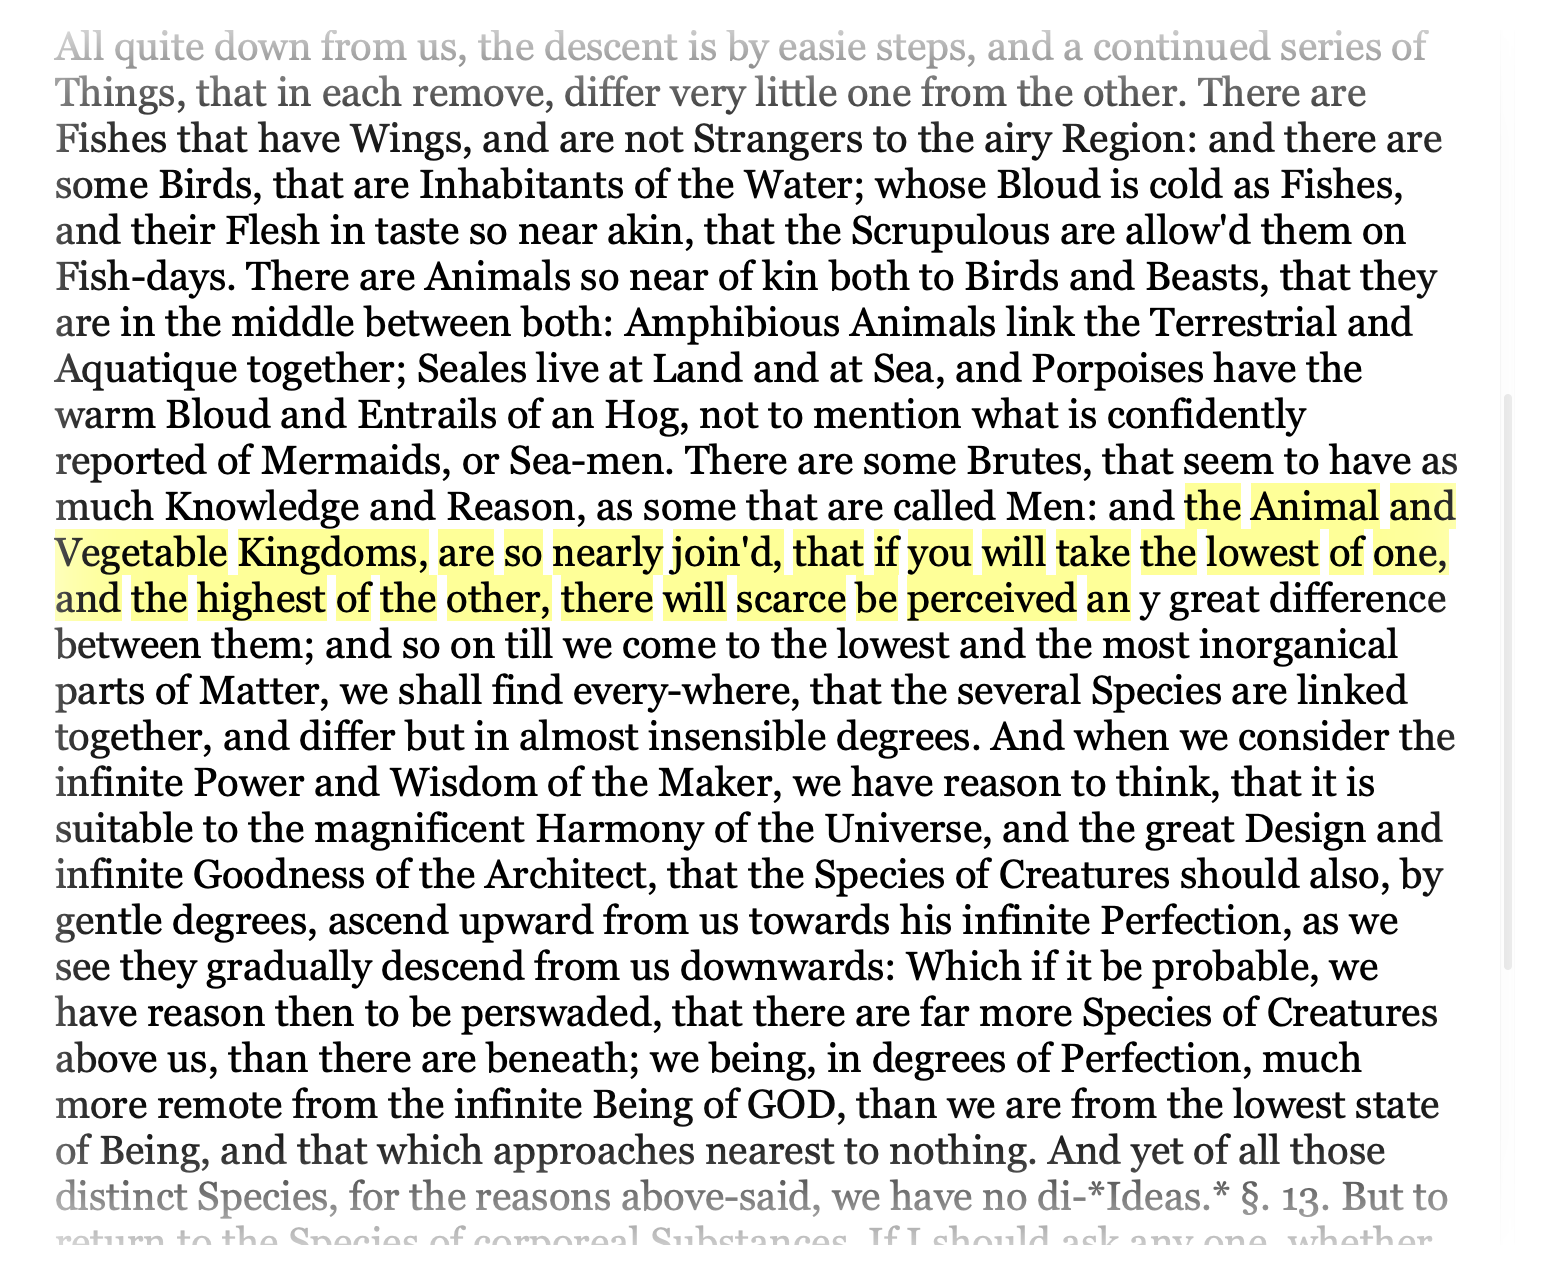
\includegraphics[width=\linewidth,clip,trim={0 5cm 0 0}]{images/quote.png}
        }
        \only<3>{
          \href{https://gallica-kaiku.rahtiapp.fi/?eccoId=1702800107&offsetStart=357168&offsetEnd=357338}{1720 - The spectator}
          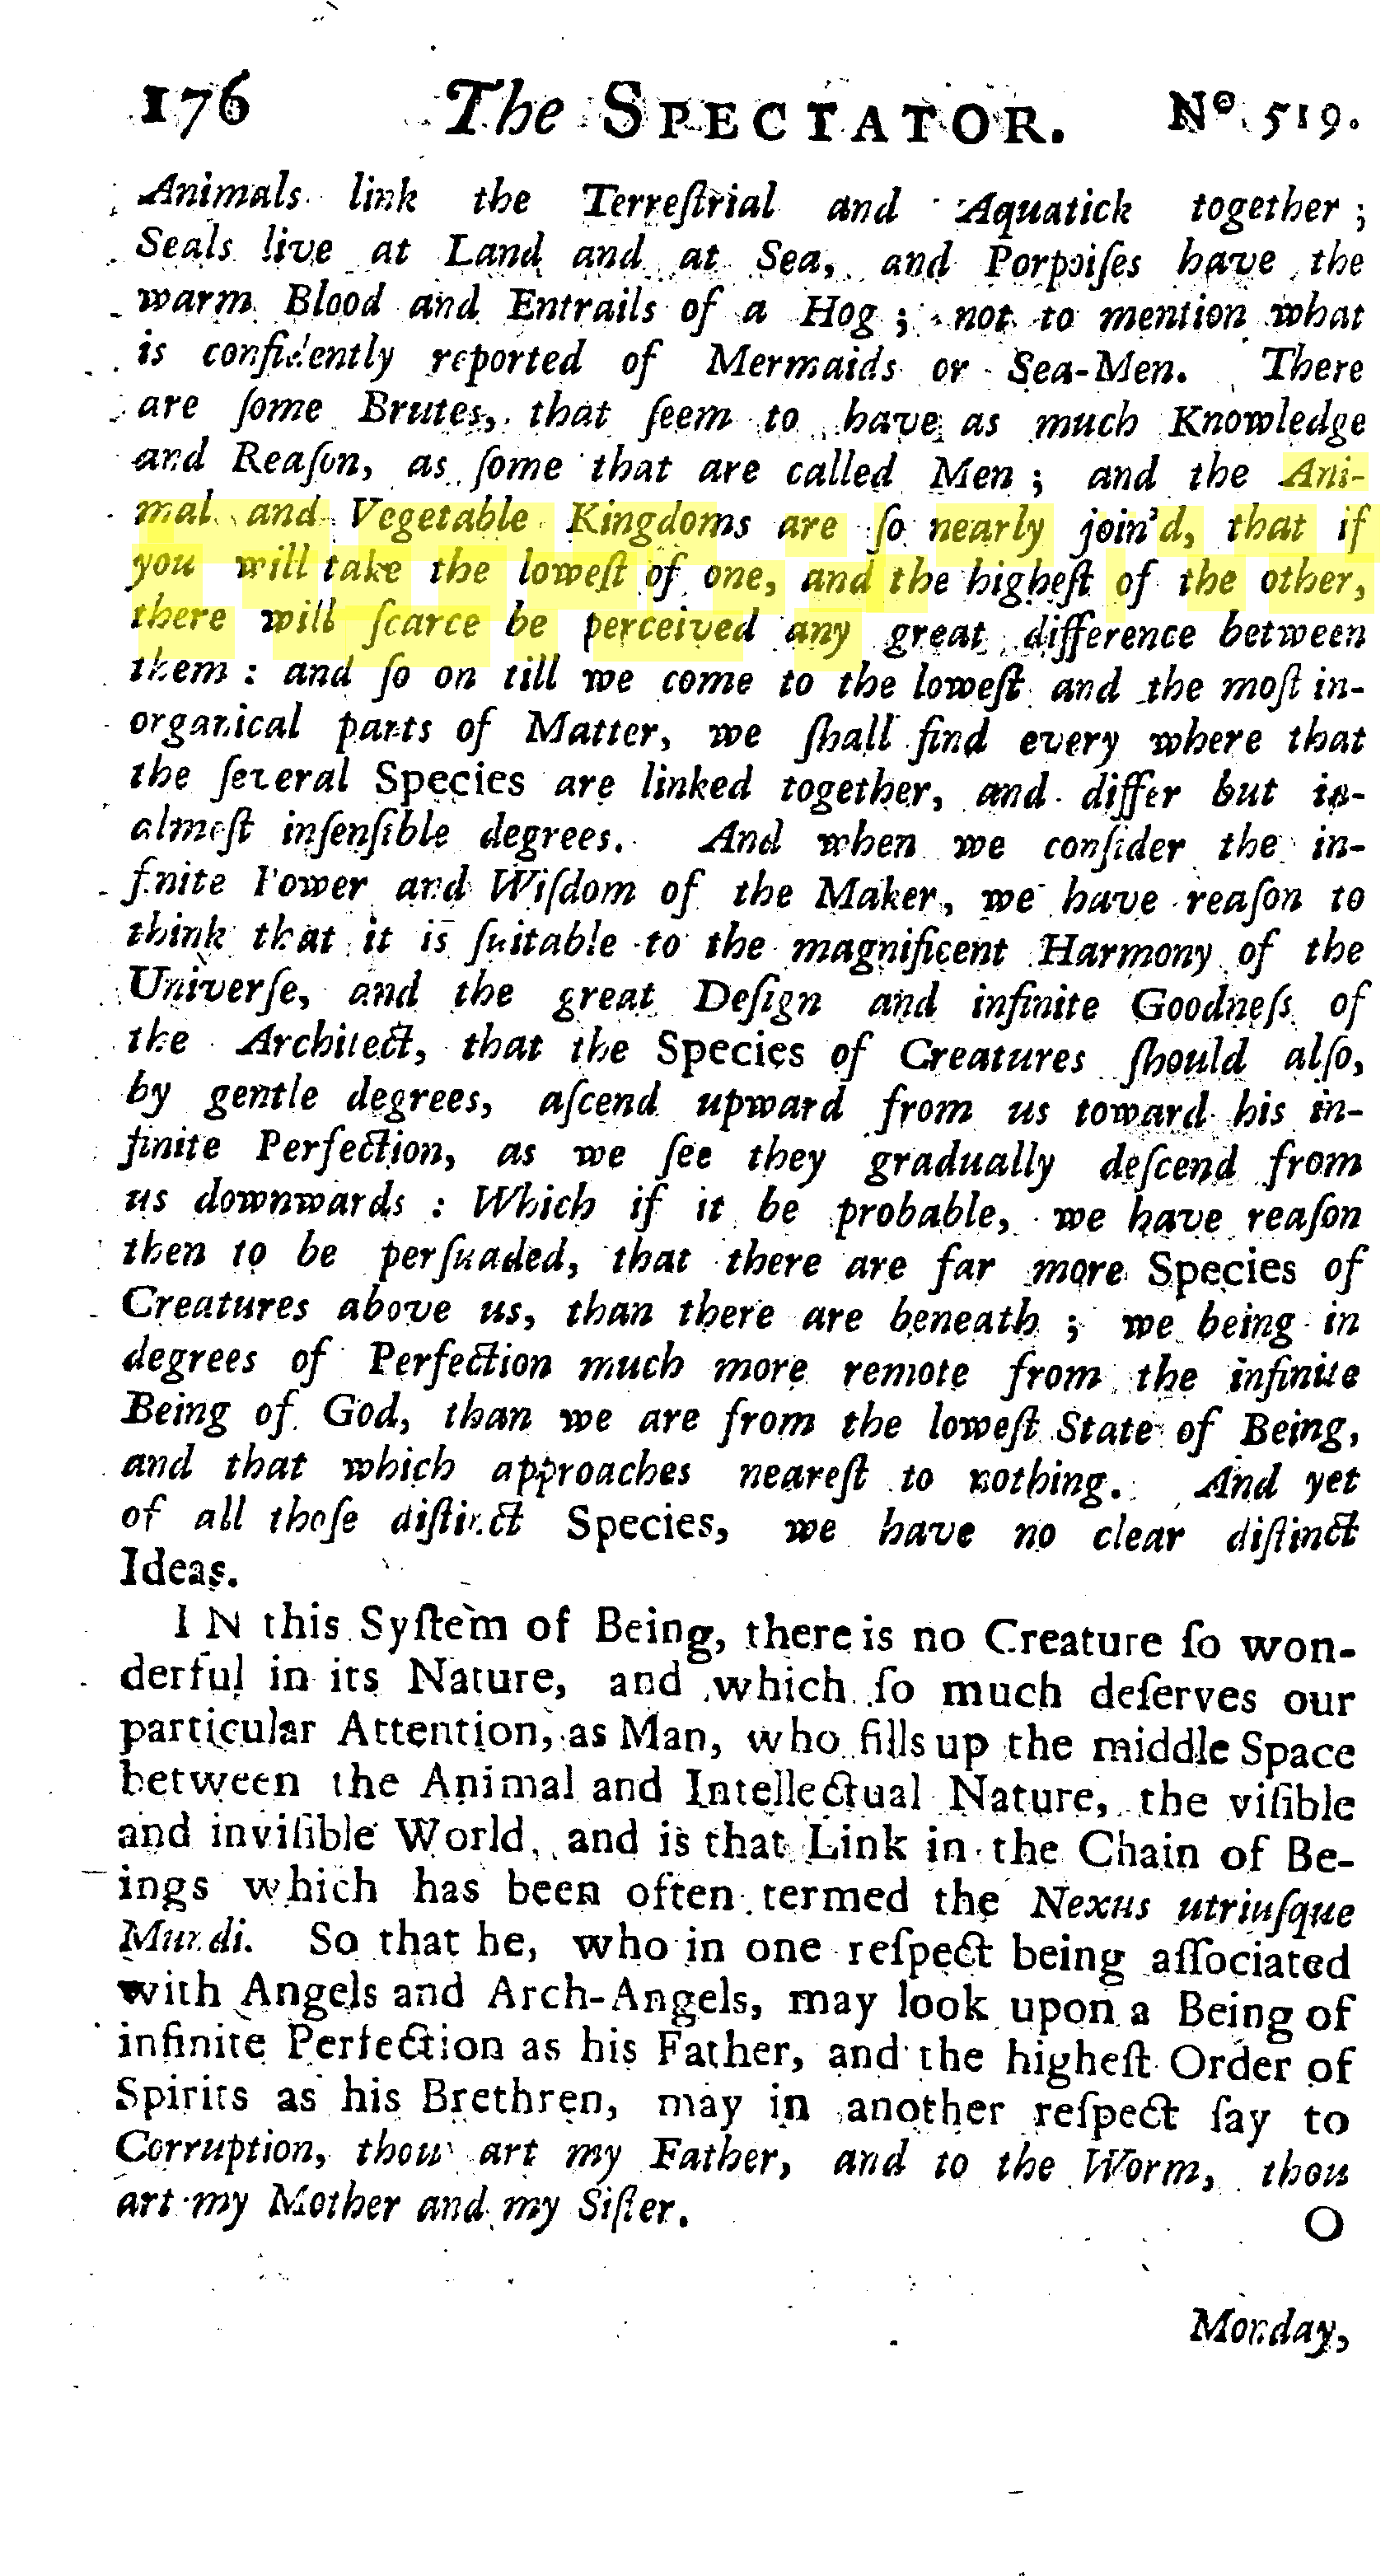
\includegraphics[width=\linewidth,height=\textheight,keepaspectratio,clip,trim={0 12cm 0 0}]{images/blast_hit.png}
          }
        \end{column}
      \end{columns}
      \end{frame}
      
\againframe<3>{locke}

% \begin{frame}
%   \frametitle{Unique Semantic Search Hits}
%   \begin{columns}
%     \begin{column}{0.45\textwidth}
%        \begin{block}{Paraphrase}
%         \small
%         ``in the vegetable and animal tribes belong- ing to the earth, and have discovered that the lowest of the animal species and the highest of the vegetable approx- imate so near to each other, that the difference betweenk the two can scarcely be perceived; but this is the very  summit of their researches; they are unable to trace the  connection of things any further, and reft satisfied in ad- mitting that The chain continues, but its''
%       \end{block}
%     \end{column}
%     \begin{column}{0.49\textwidth}
%       \href{https://gallica-kaiku.rahtiapp.fi/?eccoId=1015500300&offsetStart=715621&offsetEnd=716054}{\small Plato, 1793 - The cratylus, Phædo, Parmenides and Timæus}
%         {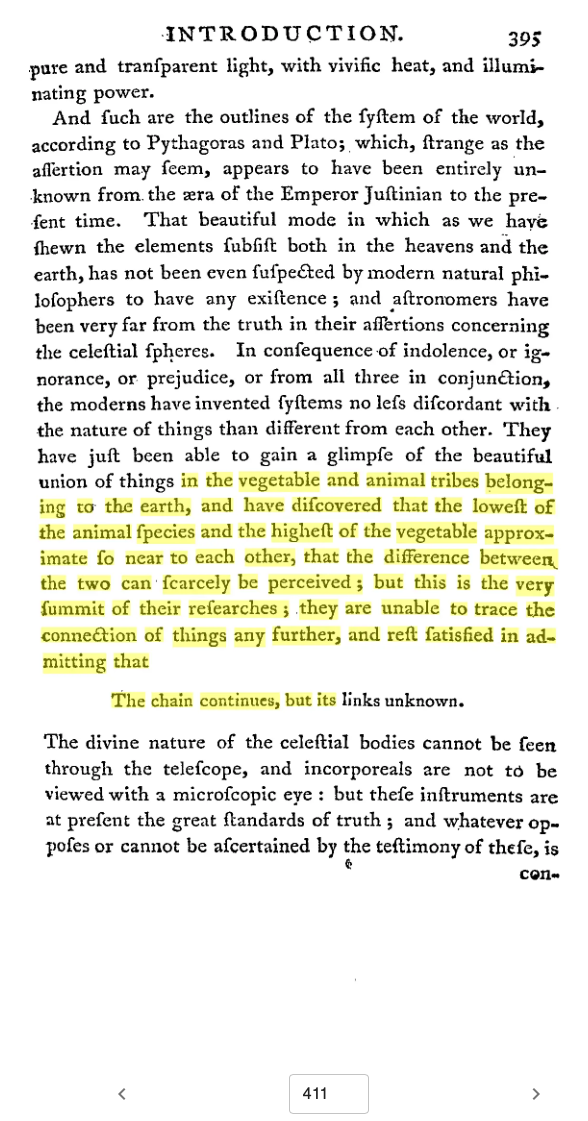
\includegraphics[width=0.9\textwidth,keepaspectratio,clip,trim={0 8cm 0 12cm}]{images/semantic_hit.png}}
%     \end{column}
%   \end{columns}
%   \end{frame}

  \begin{frame}
  \frametitle{Unique Semantic Search Hits}
  \begin{columns}
    \begin{column}{0.45\textwidth}
       \begin{block}{Topical Match}
        \small
        'vegetable kingdoms seem to- be so essentially separated, that we cannot even imagine- the leaR approximation of the one to the other. Thlole- naturalilts, indeed,, who have foppofed the ditiuaion- between animals and vegetables to consist in any thing- else than what we have already mentioned, have found- themselves greatly embarrassed, and have generally- agreed, that it was extremely difficult, if not impolfible,- to fetttle'
      \end{block}
    \end{column}
    \begin{column}{0.49\textwidth}
      \begin{center}
        \href{https://gallica-kaiku.rahtiapp.fi/?eccoId=1741200102&offsetStart=141008&offsetEnd=141430}{\small 1797 - Encyclopædia Britannica}
        {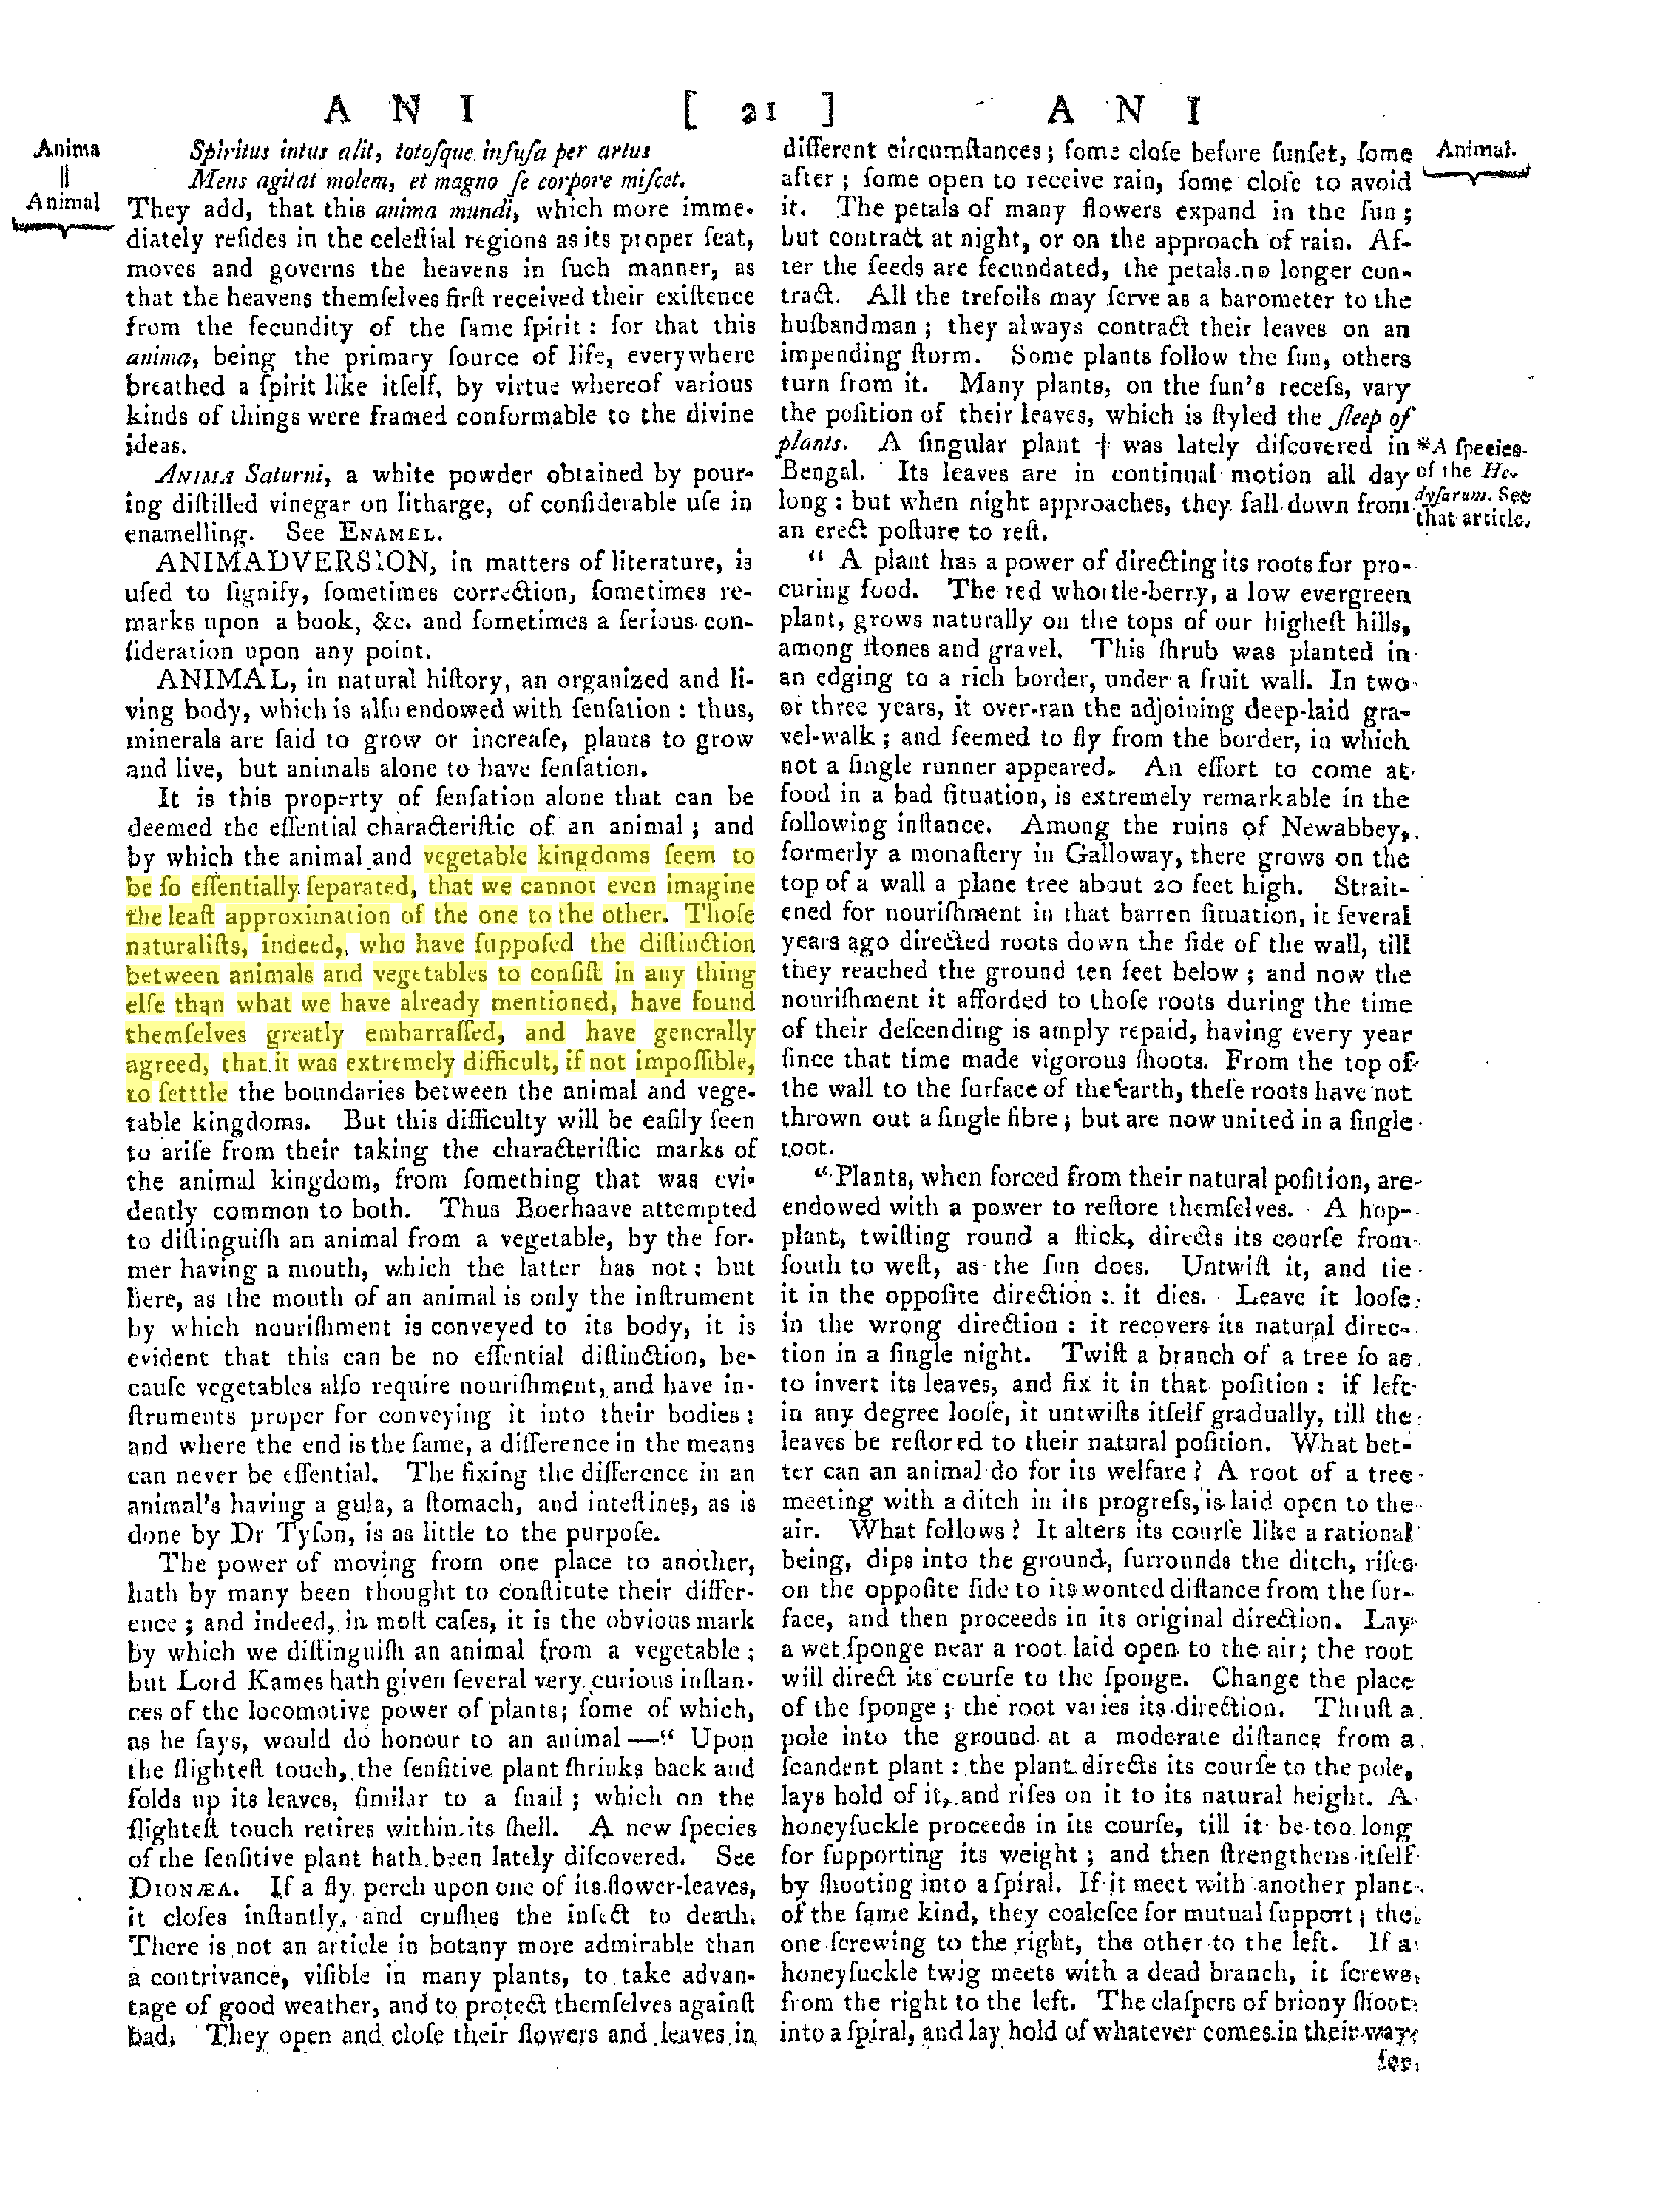
\includegraphics[width=\textwidth,height=0.7\textheight,keepaspectratio,clip,trim={1.2cm 12cm 10cm 6cm}]{images/topical_match.png}}
      \end{center}
      \end{column}
  \end{columns}
  \end{frame}


  \begin{frame}
    \frametitle{Unique Semantic Search Hits}
    \begin{columns}
      \begin{column}{0.45\textwidth}
         \begin{block}{Meaning Match}
          \small
          ``ach to animals; and that this similarity, as well as the- difficulty of fixing the precise boundaries by which. these two great.- kingdoms of nature are limited, are diret. cbnfequences of the or-- ganization of vegetables. It. is owing to their organic flruaure- alone, that plants and animals are capable of affording reciprocal- nourishment to each other. This organic firuaure, though greatly- diversified''
        \end{block}
      \end{column}
      \begin{column}{0.49\textwidth}
        \href{https://gallica-kaiku.rahtiapp.fi/?eccoId=1015500300&offsetStart=715621&offsetEnd=716054}{\small Smellie, William (1740-1795) 1790 - The philosophy of natural history}
          {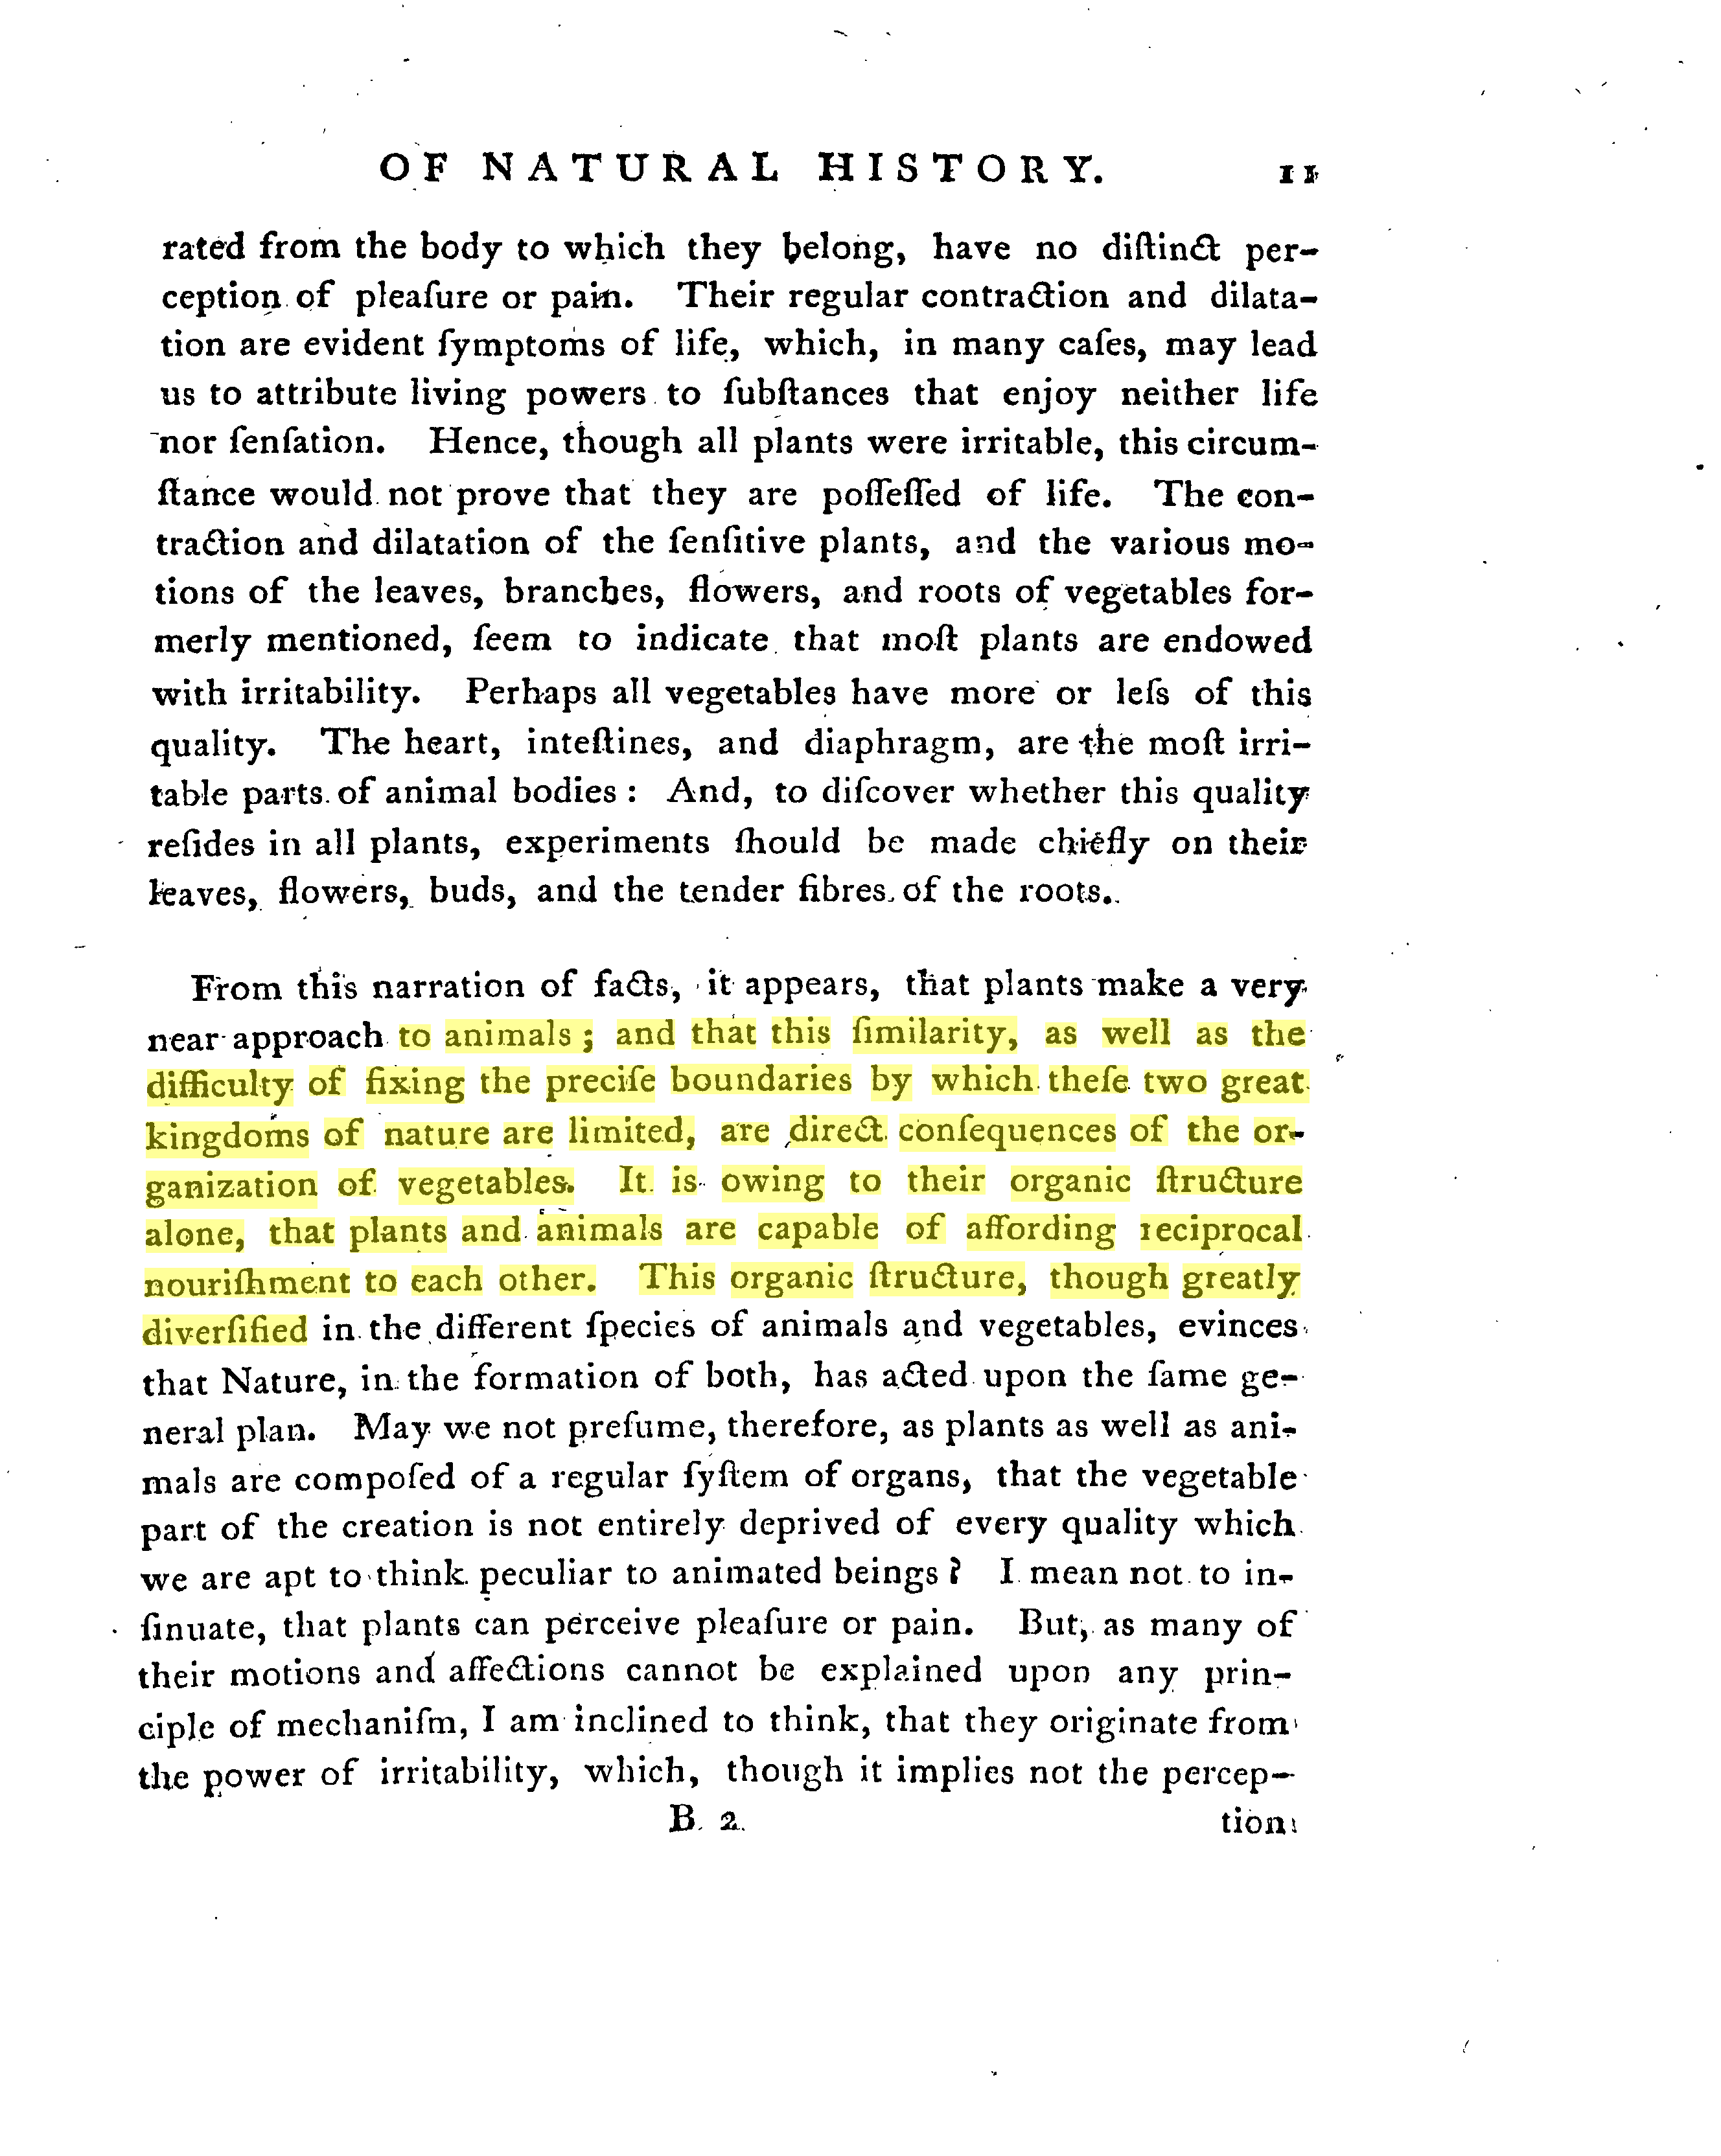
\includegraphics[width=0.9\textwidth,keepaspectratio,clip,trim={1.5cmcm 8cm 5cm 8cm}]{images/meaning_match.png}}
      \end{column}
    \end{columns}
    \end{frame}
  

\section{Discussion Questions}

\begin{frame}
  \frametitle{Questions for future work}
  Lexical Text Reuses
  \begin{itemize}
    \item Handling fragmented/overlapping reuses
    \item Managing metadata from different sources
    \item Building more interfaces for custom tasks
  \end{itemize}
  Semantic Text Reuses
  \begin{itemize}
    \item Calibrate similarity scores across queries
    \item Identify region of similarity withing a hit
    \item Filter out topical matches
  \end{itemize}
  

\end{frame}
\end{document}  